\documentclass[a4paper,12pt]{article}

\usepackage[top=3cm, bottom=2cm, left=3cm, right=2cm]{geometry}
\usepackage[utf8]{inputenc}
\usepackage[portuguese]{babel}
\usepackage{graphicx}
\graphicspath{{./planos_execucao/}}
\usepackage{subfig}
\usepackage{booktabs}
\usepackage{multirow}
\usepackage{verbatim}

\usepackage{float}
\usepackage{morefloats}
\floatstyle{ruled}
\newfloat{program}{thp}{lop}
\floatname{program}{Query}

\title{Tecnologia de Bases de Dados\\
Otimização de Interrogações}

\author{André Fernandes (ei03107) \and Pedro Batista (ext10392)}

\begin{document}

\maketitle

Para a Query~\ref{sql:1-a} observamos que o caso B tem um custo
ligeiramente maior que o caso A, pois foram adicionadas chaves estrangeiras.
Já no caso C observamos um custo bem menor, pois o filtro é aplicado
somente na chave, necessitando dessa forma buscar na tabela apenas as linhas que
atendem a condição.

\begin{program}
   \verbatiminput{respostas/1-a.sql}
   \caption{Pergunta sobre seleção 1.a.}
   \label{sql:1-a}
\end{program}

\begin{figure}[thp]
   \begin{center}
      \subfloat[Situação A]{\label{fig:plano_1-a_A}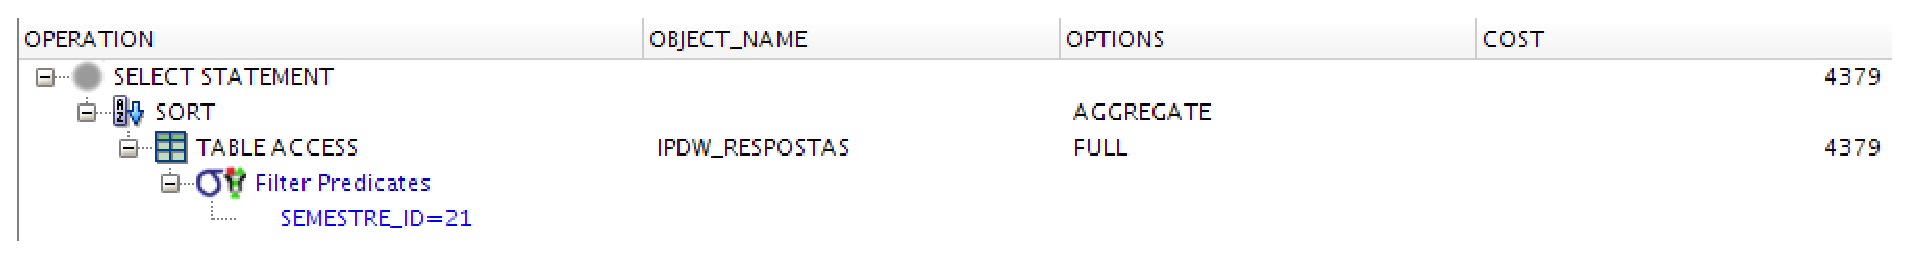
\includegraphics[width=1\textwidth]{1-a_A}}\\
      \subfloat[Situação B]{\label{fig:plano_1-a_B}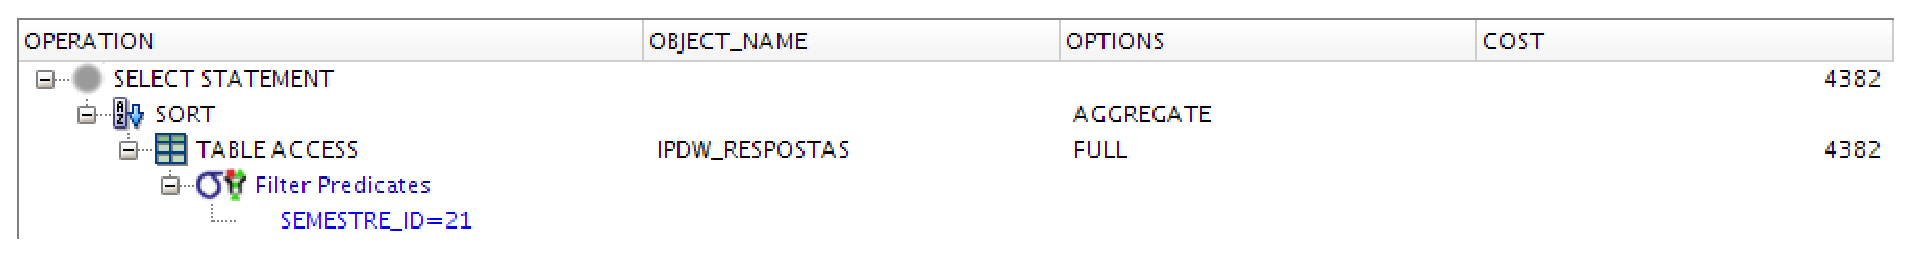
\includegraphics[width=1\textwidth]{1-a_B}}\\
      \subfloat[Situação C]{\label{fig:plano_1-a_C}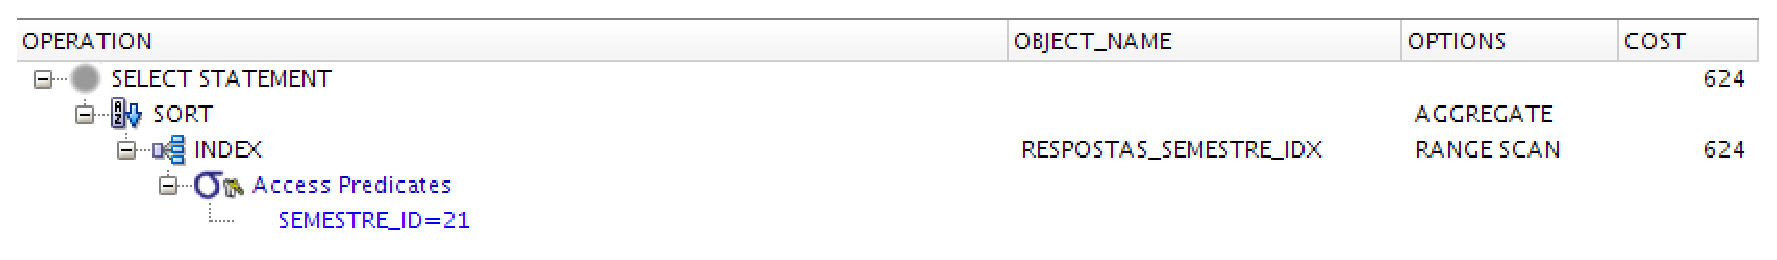
\includegraphics[width=1\textwidth]{1-a_C}}
   \end{center}
   \caption{Plano de execução para a Query \ref{sql:1-a}.}
   \label{fig:plano_1-a}
\end{figure}

Na Query~\ref{sql:1-b} entre os casos A e B também foi observado um aumento
devido a chave estrangeira. No caso C observamos um custo bem menor
do que o no caso C da Query~\ref{sql:1-a}, pois a seletividade de disciplina\_id
é bem maior que a de semestre\_id.

\begin{program}
   \verbatiminput{respostas/1-b.sql}
   \caption{Pergunta sobre seleção 1.b.}
   \label{sql:1-b}
\end{program}

\begin{figure}[hpt]
   \begin{center}
      \subfloat[Situação A]{\label{fig:plano_1-b_A}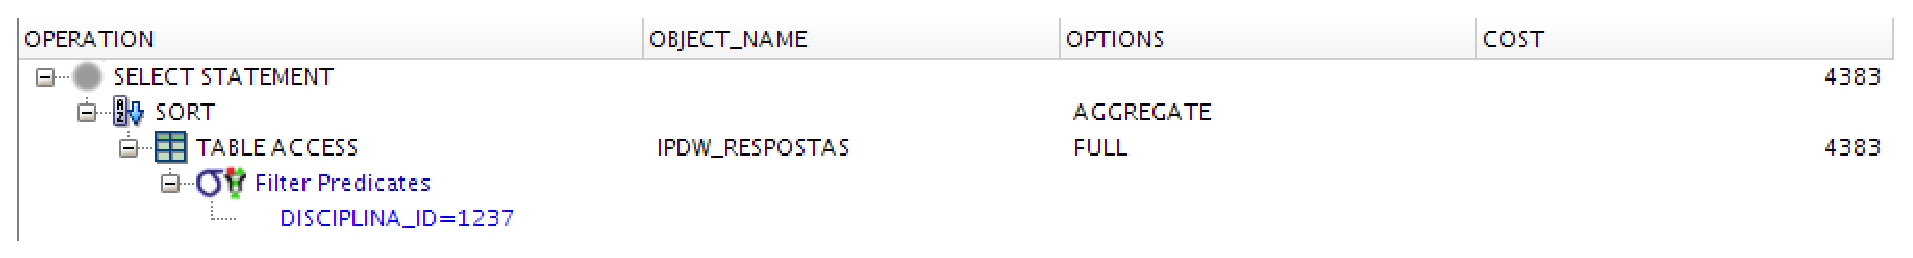
\includegraphics[width=1\textwidth]{1-b_A}}\\
      \subfloat[Situação B]{\label{fig:plano_1-b_B}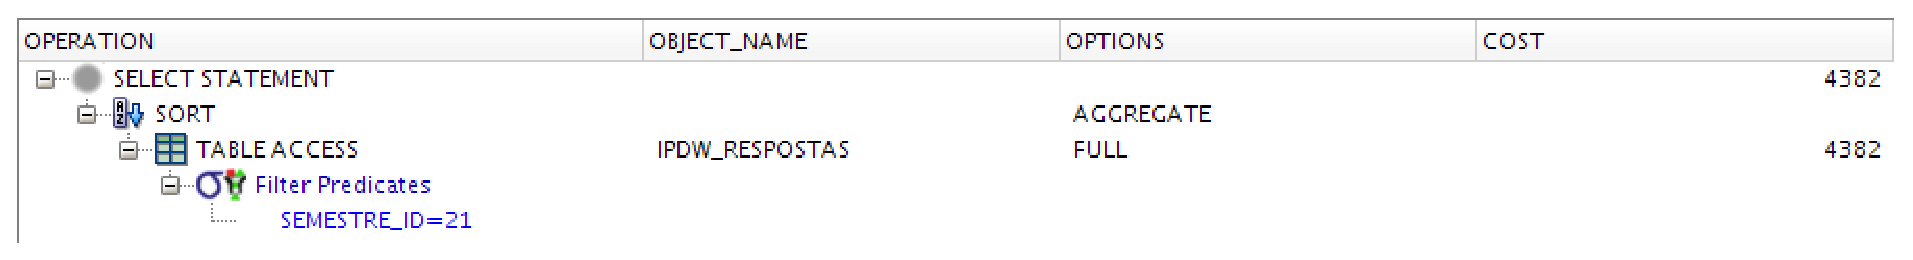
\includegraphics[width=1\textwidth]{1-b_B}}\\
      \subfloat[Situação C]{\label{fig:plano_1-b_C}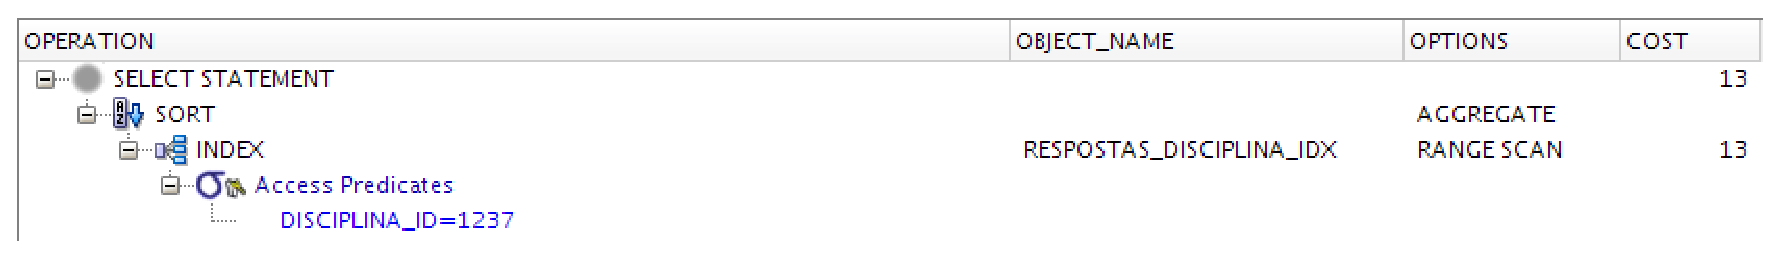
\includegraphics[width=1\textwidth]{1-b_C}}
   \end{center}
   \caption{Plano de execução para a Query \ref{sql:1-b}.}
   \label{fig:plano_1-b}
\end{figure}

Para a Query~\ref{sql:1-c} nos casos A e B a análise anterior também se aplica.
No caso C observamos que não foi necessário fazer um acesso completo a tabela ipdw\_respostas,
pois um index foi criado em sua coluna semestre\_id. Dessa forma se tornou viável a
a pesquisa sequencial através de um Nested Loop ao invés de um Hash Join.

\begin{program}
   \verbatiminput{respostas/1-c.sql}
   \caption{Pergunta sobre seleção 1.c.}
   \label{sql:1-c}
\end{program}

\begin{figure}[hpt]
   \begin{center}
      \subfloat[Situação A]{\label{fig:plano_1-c_A}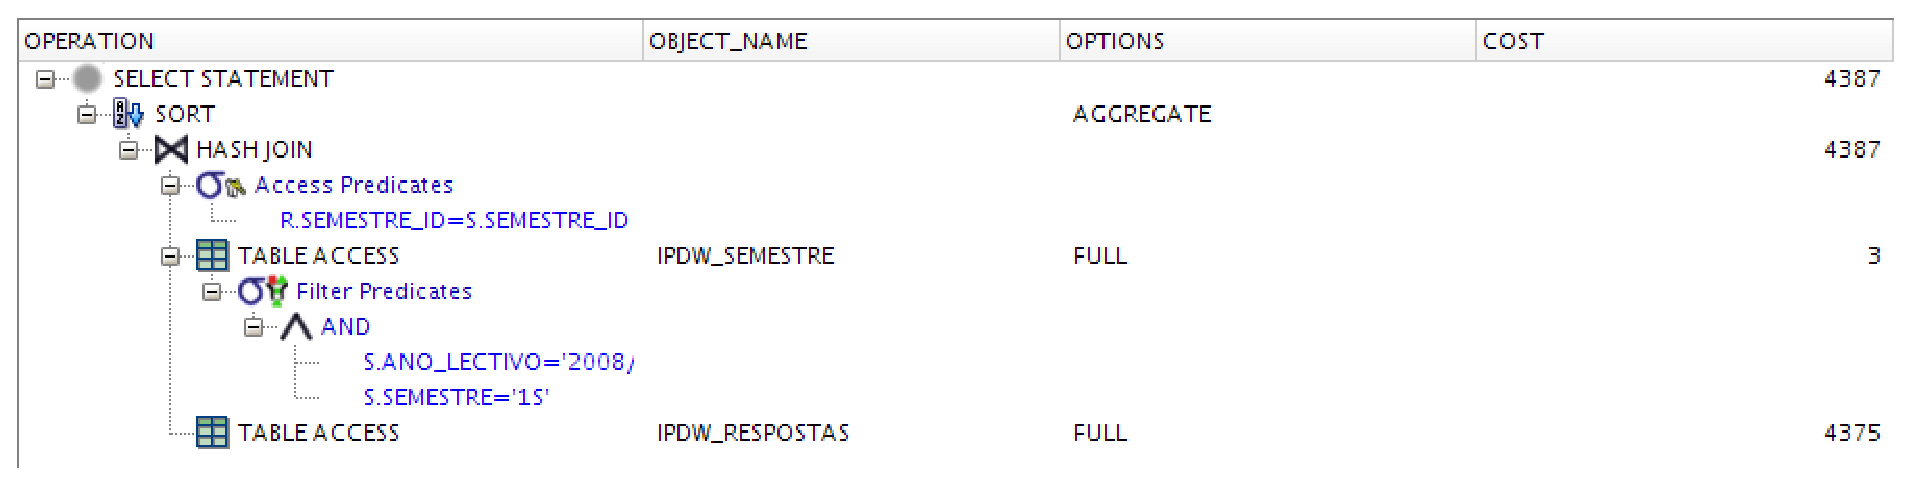
\includegraphics[width=1\textwidth]{1-c_A}}\\
      \subfloat[Situação B]{\label{fig:plano_1-c_B}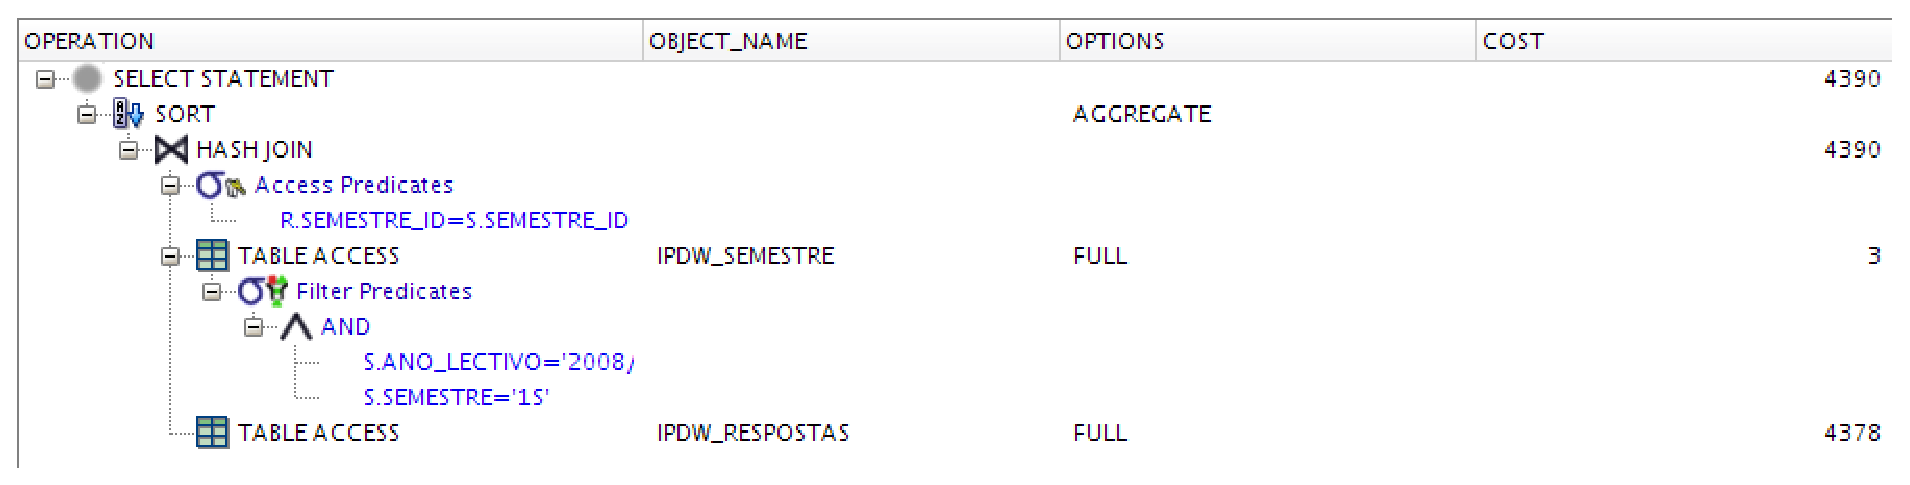
\includegraphics[width=1\textwidth]{1-c_B}}\\
      \subfloat[Situação C]{\label{fig:plano_1-c_C}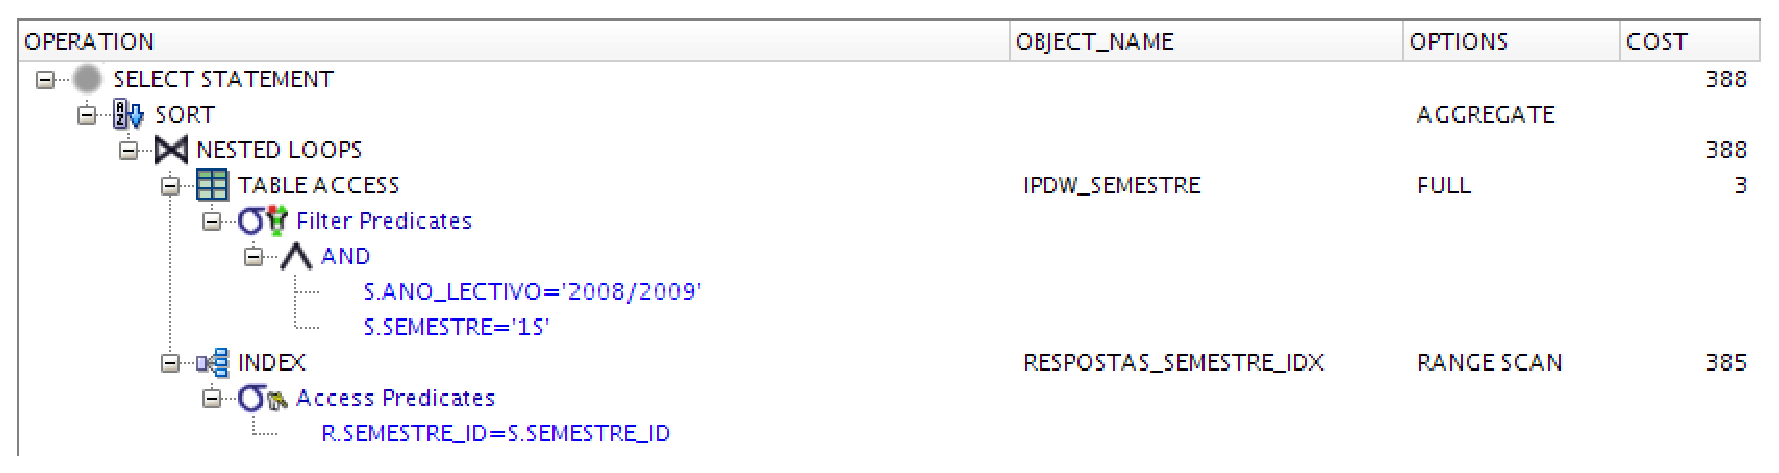
\includegraphics[width=1\textwidth]{1-c_C}}
   \end{center}
   \caption{Plano de execução para a Query \ref{sql:1-c}.}
   \label{fig:plano_1-c}
\end{figure}

Na Query~\ref{sql:2-a} notamos o efeito da adição do index na coluna disciplina\_id
da tabela respostas, e na sigla da tabela disciplina. Pois foi possível selecionar
os ids das disciplinas de interesse e fazer um Nested Loop utilizando apenas
indexes da tabela respostas. Dessa forma apenas valores do resultado foram
acessados na tabela respostas utilizando os ROWID adquiridos no Nested Loop.
O que minimizou o número de acessos.

\begin{program}
   \verbatiminput{respostas/2-a.sql}
   \caption{Pergunta sobre agregação 2.a.}
   \label{sql:2-a}
\end{program}

\begin{figure}[hpt]
   \begin{center}
      \subfloat[Situação A]{\label{fig:plano_2-a_A}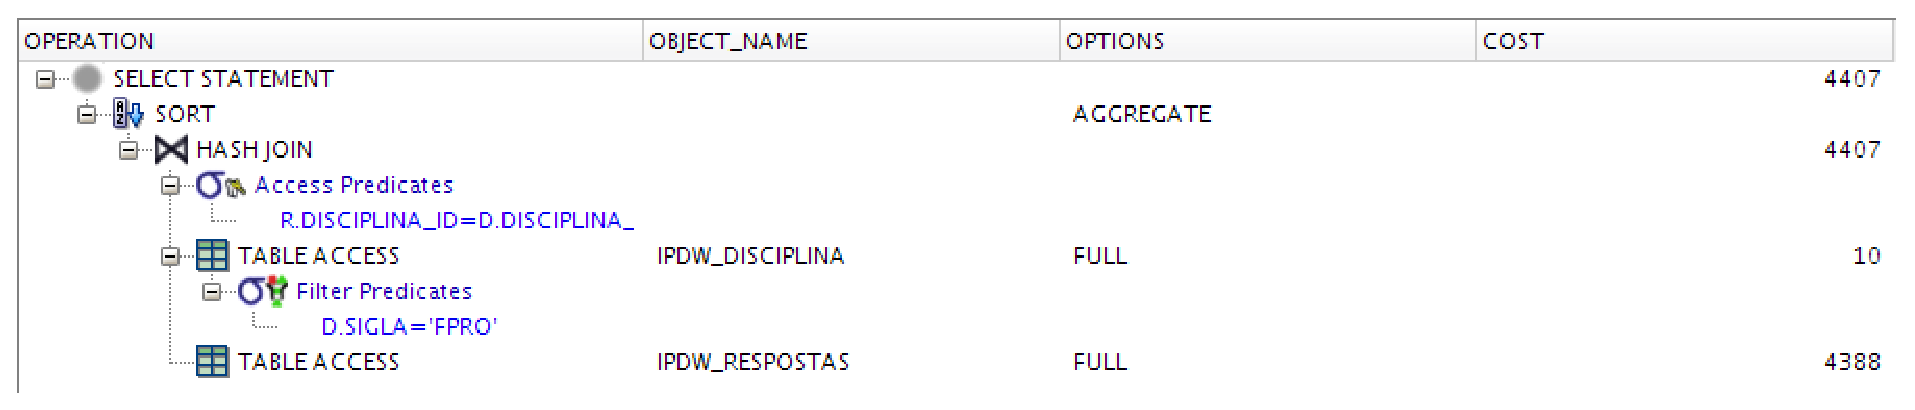
\includegraphics[width=1\textwidth]{2-a_A}}\\
      \subfloat[Situação B]{\label{fig:plano_2-a_B}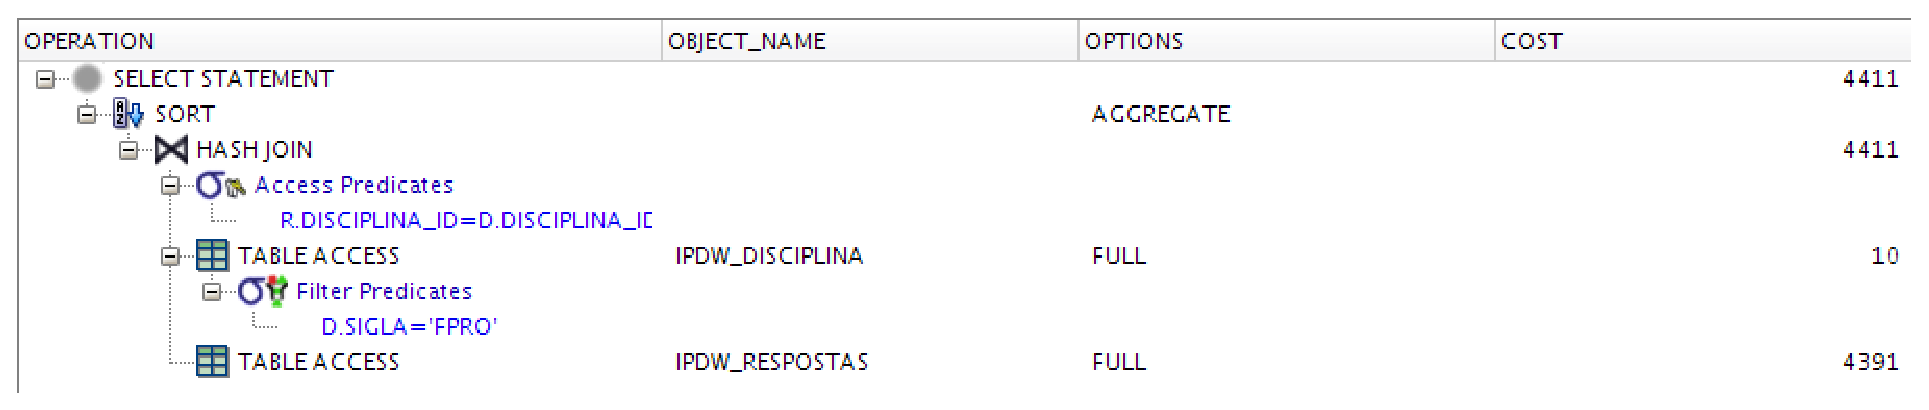
\includegraphics[width=1\textwidth]{2-a_B}}\\
      \subfloat[Situação C]{\label{fig:plano_2-a_C}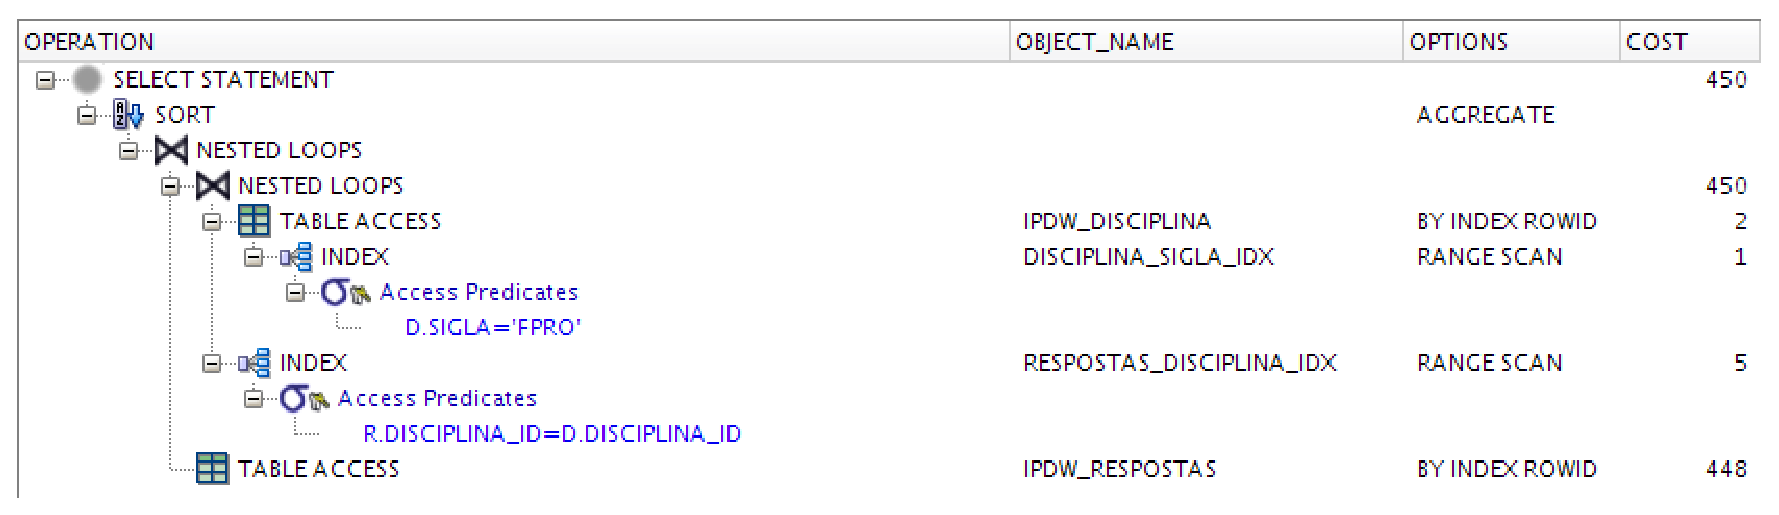
\includegraphics[width=1\textwidth]{2-a_C}}
   \end{center}
   \caption{Plano de execução para a Query \ref{sql:2-a}.}
   \label{fig:plano_2-a}
\end{figure}

Para a Query~\ref{sql:2-b} o index na coluna semestre\_id da tabela resposta
permitiu evitar um acesso completo a tabela. Pois o filtro foi feito
pelo index. Minimizando assim o volume de dados no restante do processo.

\begin{program}
   \verbatiminput{respostas/2-b.sql}
   \caption{Pergunta sobre agregação 2.b.}
   \label{sql:2-b}
\end{program}

\begin{figure}[hpt]
   \begin{center}
      \subfloat[Situação A]{\label{fig:plano_2-b_A}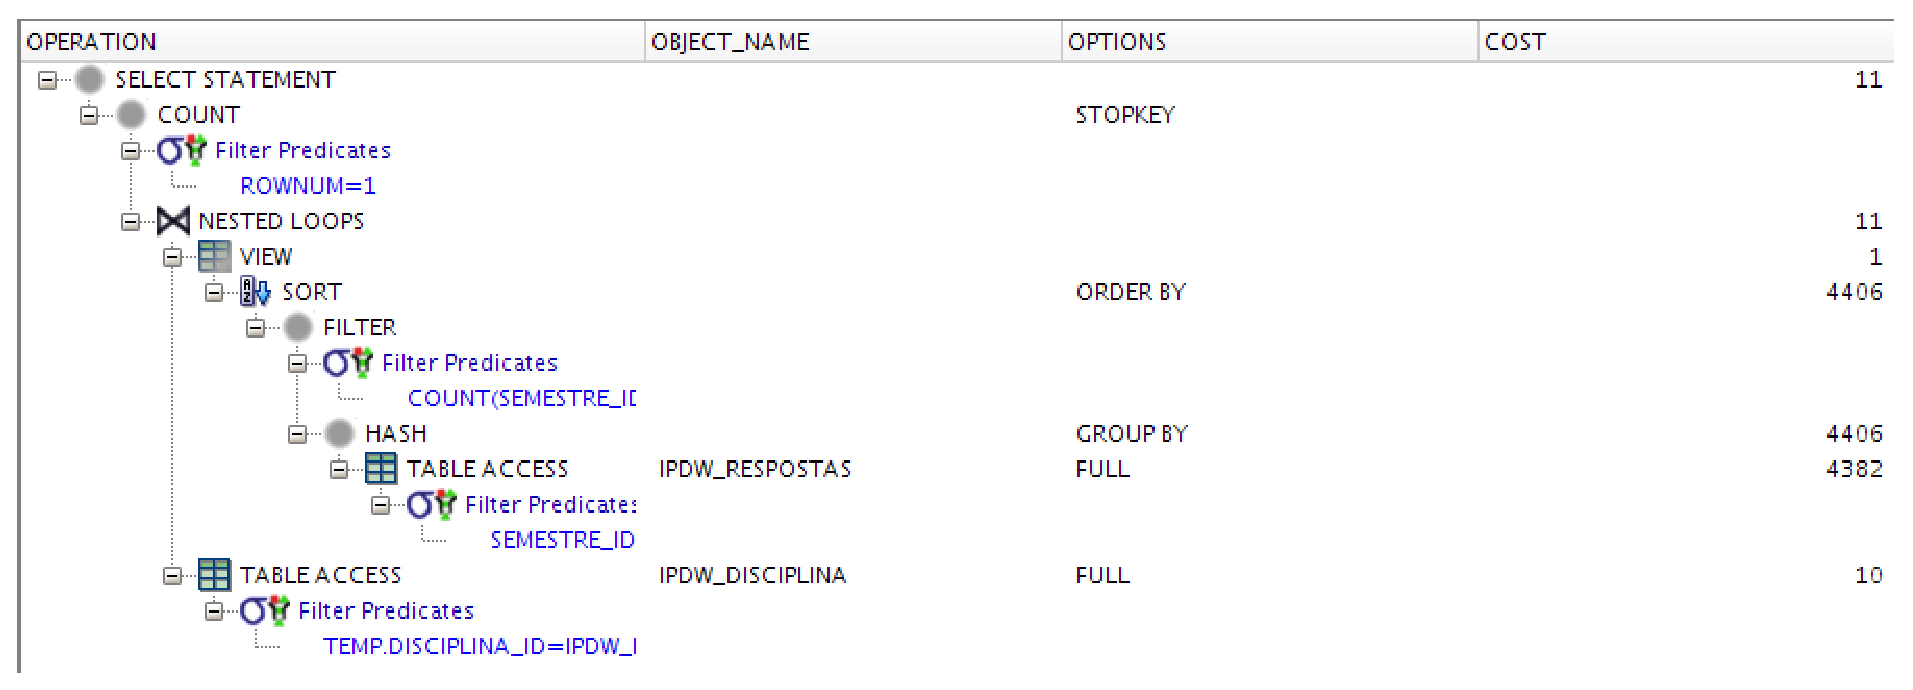
\includegraphics[width=1\textwidth]{2-b_A}}\\
      \subfloat[Situação B]{\label{fig:plano_2-b_B}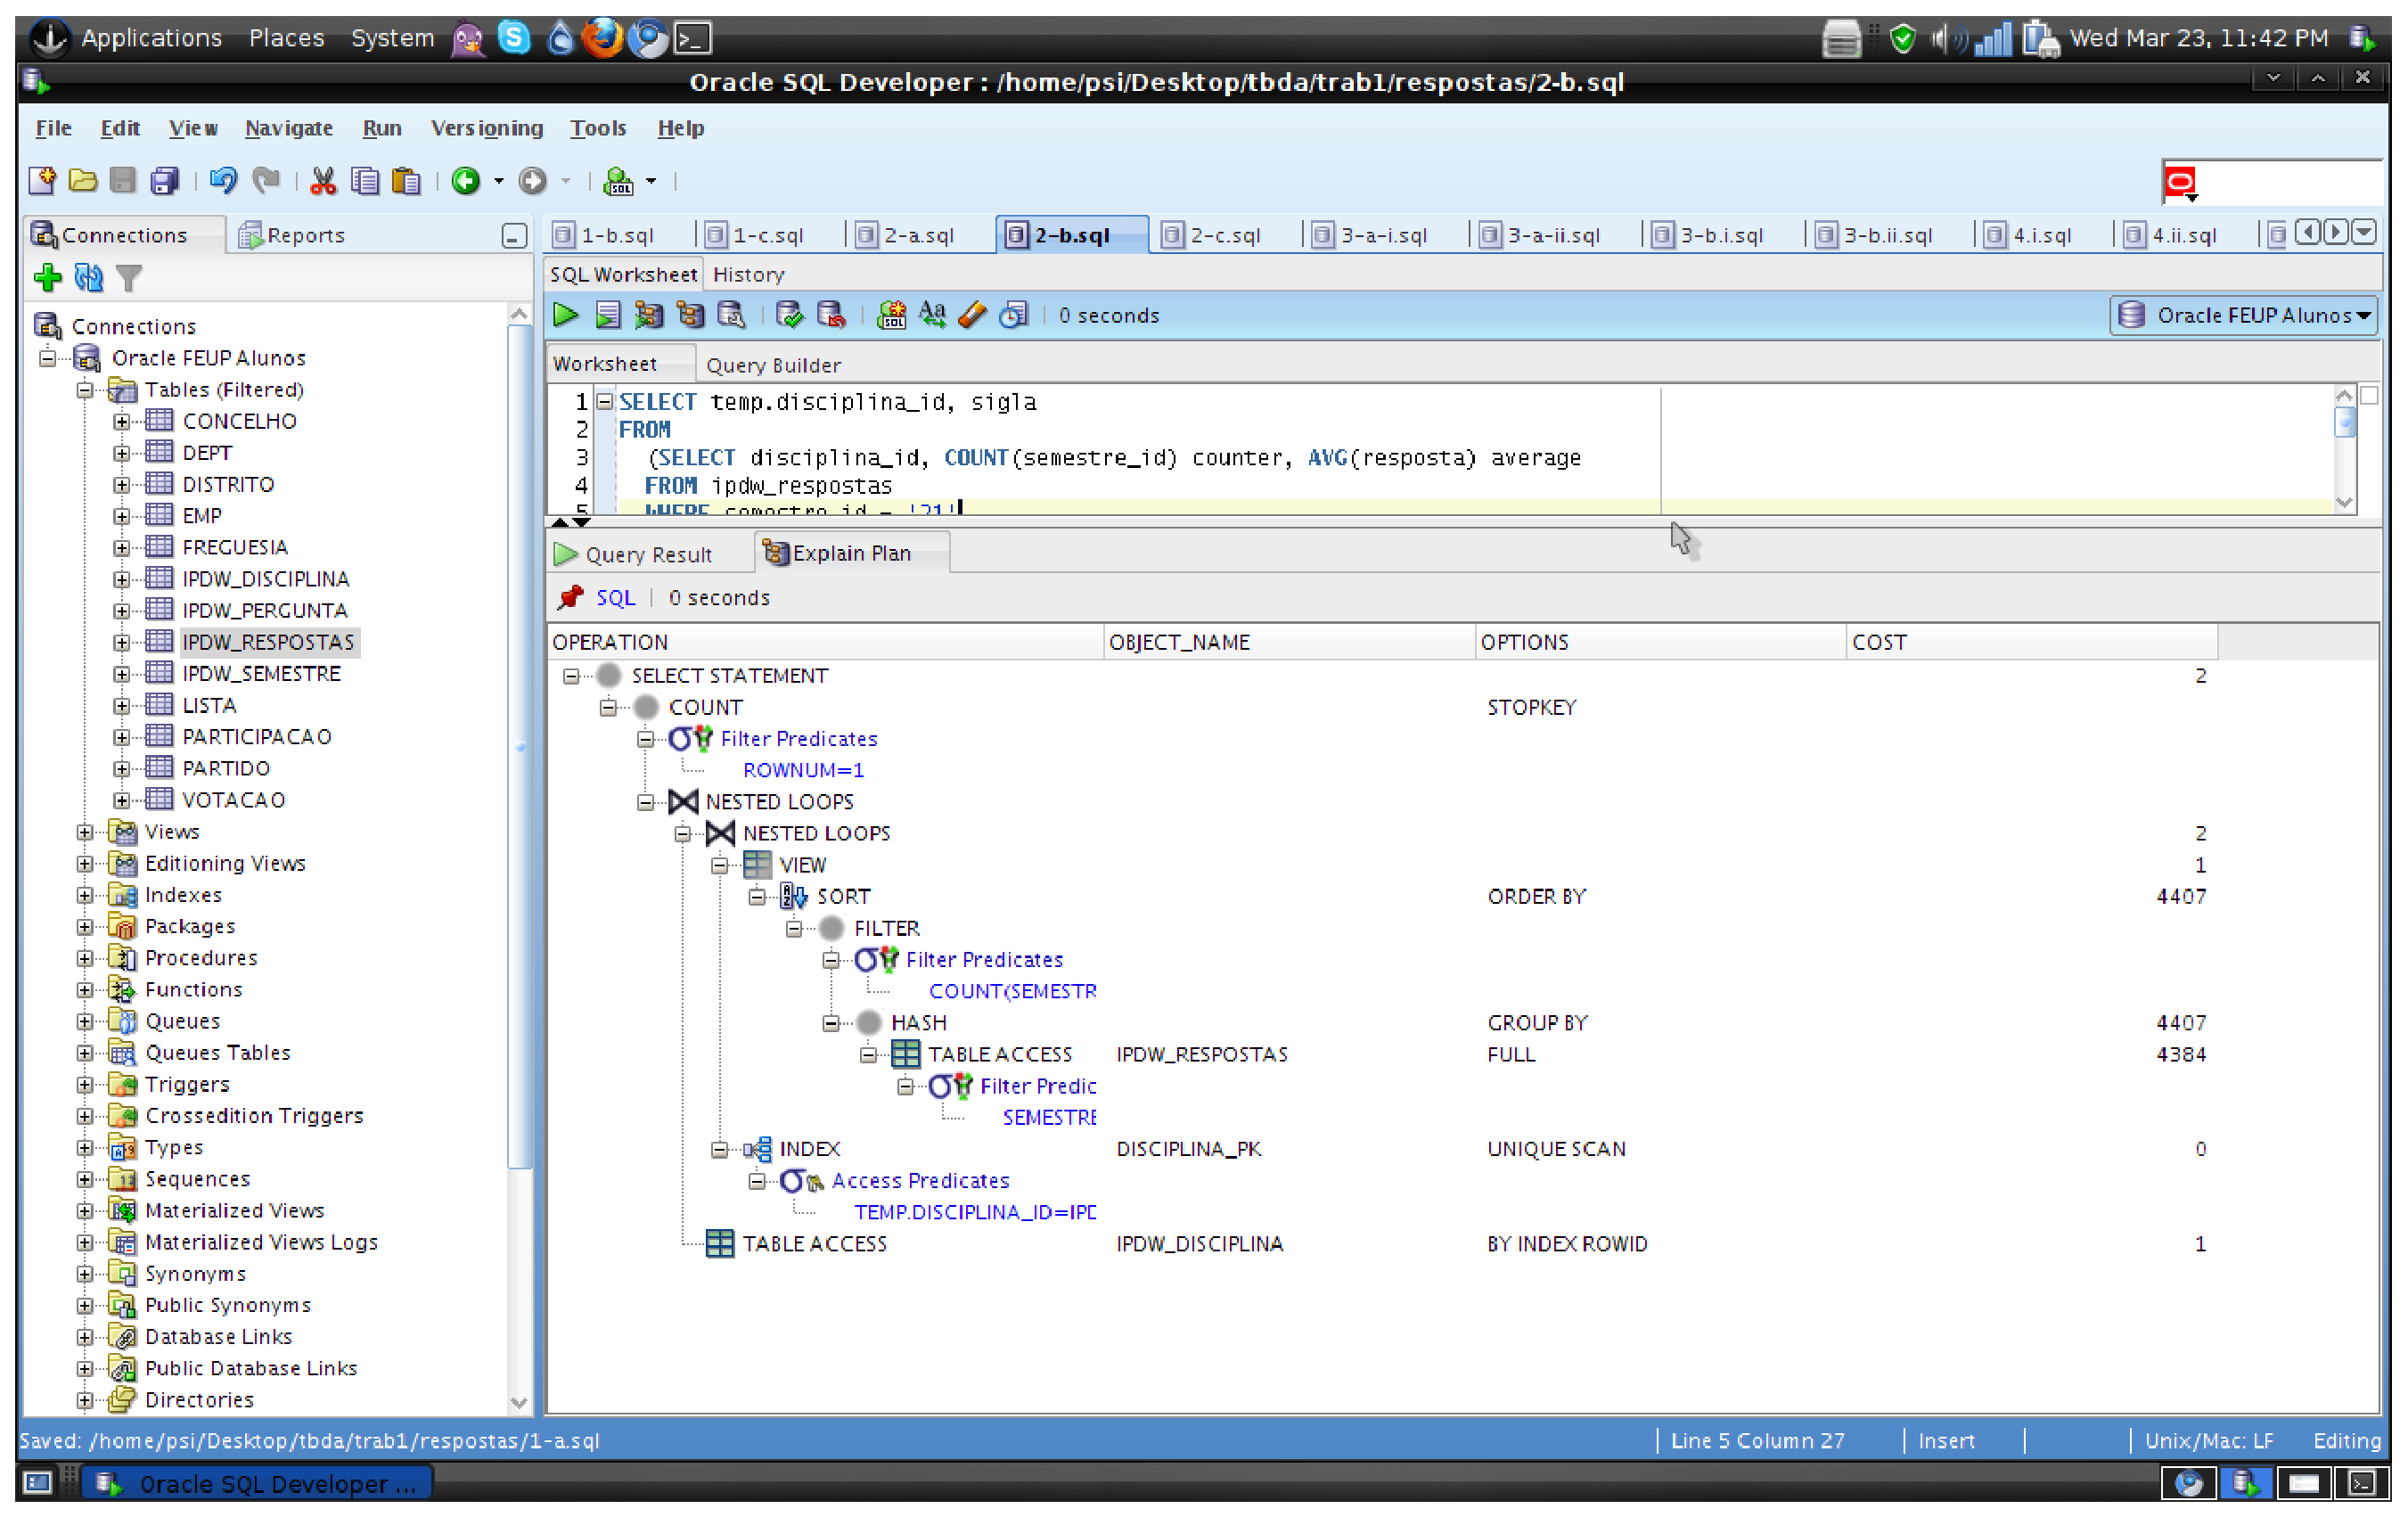
\includegraphics[width=1\textwidth]{2-b_B}}\\
      \subfloat[Situação C]{\label{fig:plano_2-b_C}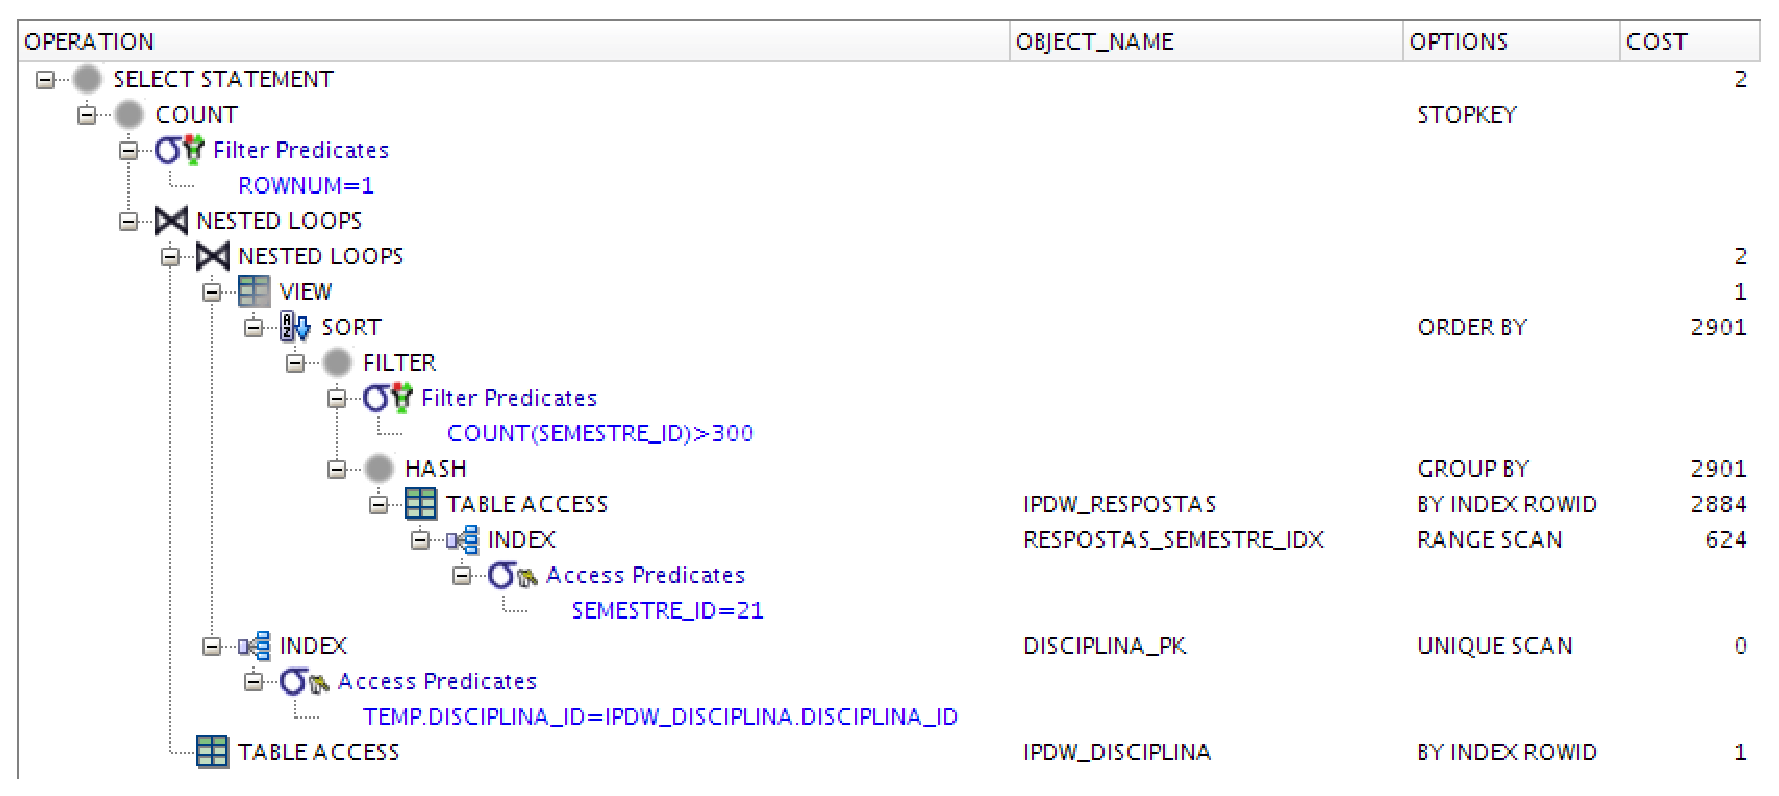
\includegraphics[width=1\textwidth]{2-b_C}}
   \end{center}
   \caption{Plano de execução para a Query \ref{sql:2-b}.}
   \label{fig:plano_2-b}
\end{figure}

Na Query~\ref{sql:2-c} os indices novamente evitaram acessos a tabela, mais uma vez
através dele foi possível fazer um filtro. Uma nova forma de utilização deste
também foi mostrada nessa situação, após filtrado, para facilitar o AND que garante
que o disciplina\_id é o 21 e que a pergunta é ``Apreciação Global'' foi formado
um BITMAP, pois dessa forma é mais fácil verificar a intercessão dos ROWID.

\begin{program}
   \verbatiminput{respostas/2-c.sql}
   \caption{Pergunta sobre agregação 2.c.}
   \label{sql:2-c}
\end{program}

\begin{figure}[hpt]
   \begin{center}
      \subfloat[Situação A]{\label{fig:plano_2-c_A}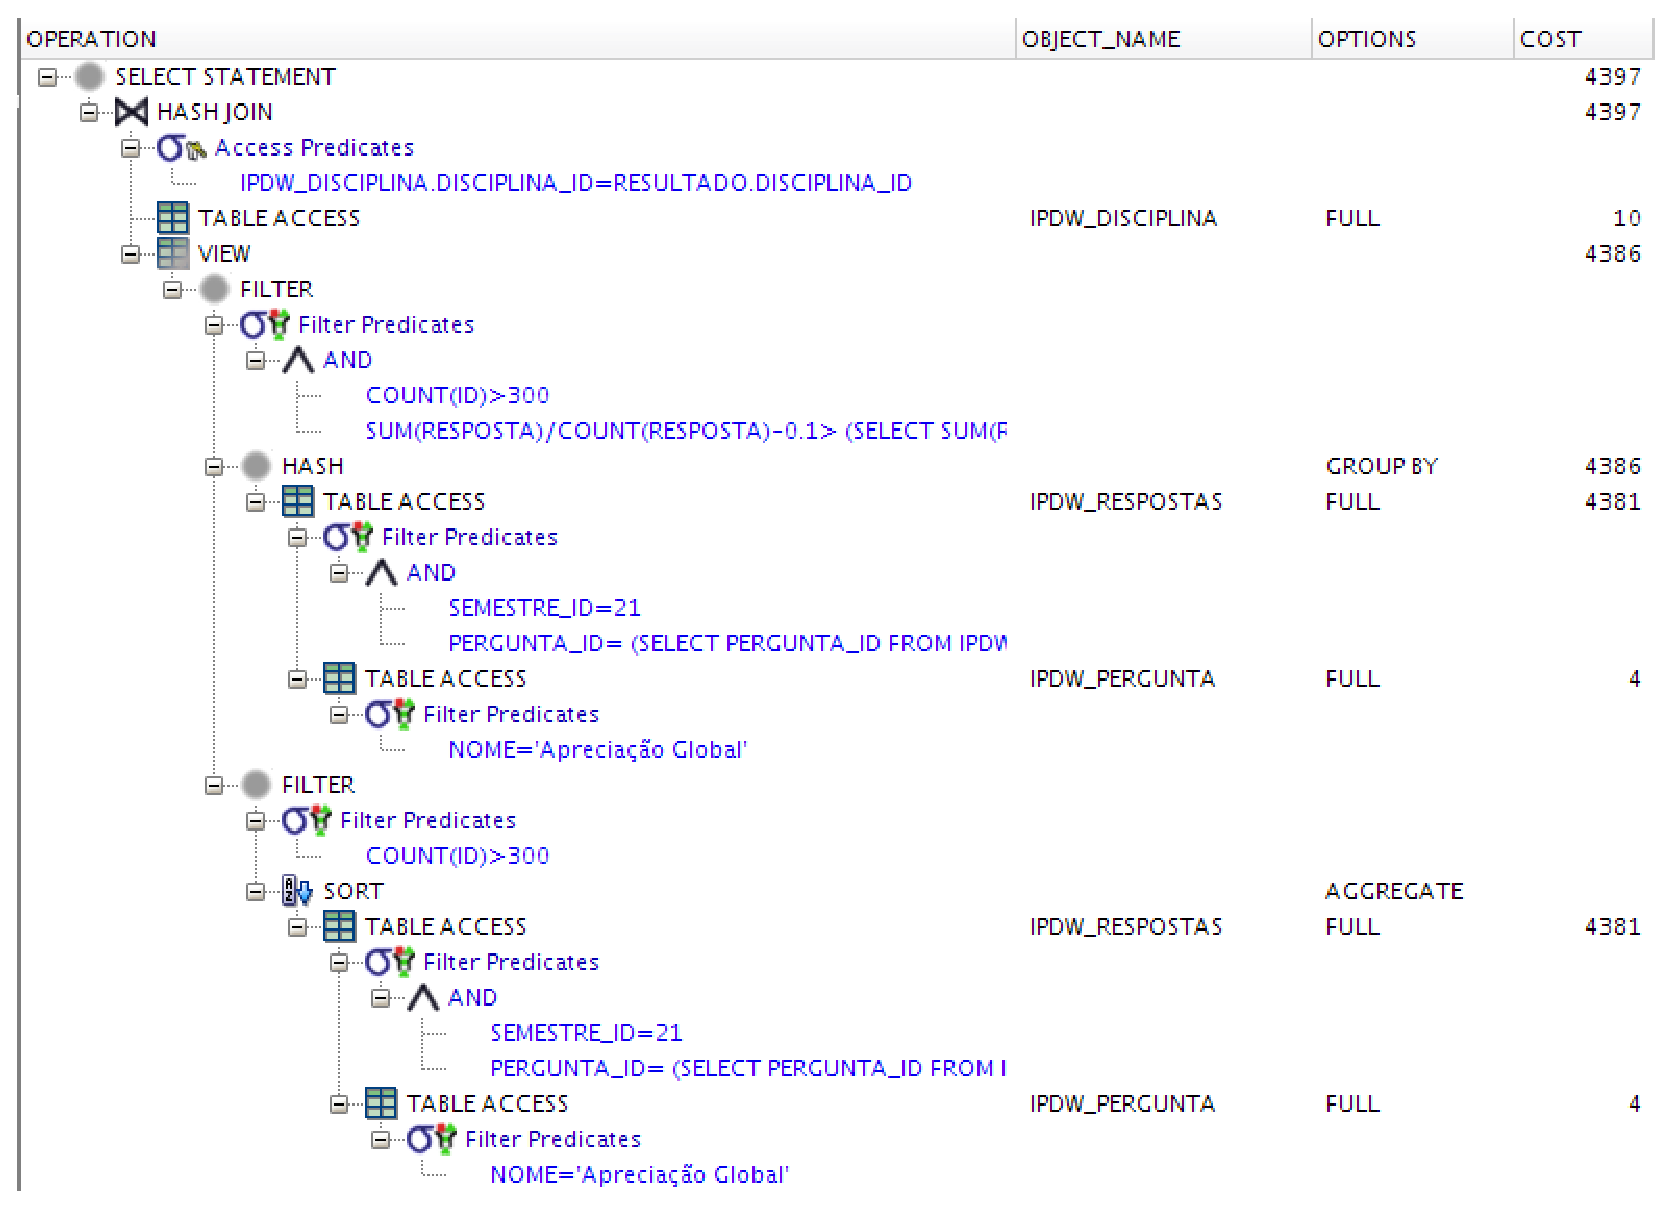
\includegraphics[width=1\textwidth]{2-c_A}}
   \end{center}
   \caption{Plano de execução para a Query \ref{sql:2-c}.}
   \label{fig:plano_2-c}
\end{figure}

\begin{figure}[hpt]
   \begin{center}
      \ContinuedFloat
      \subfloat[Situação B]{\label{fig:plano_2-c_B}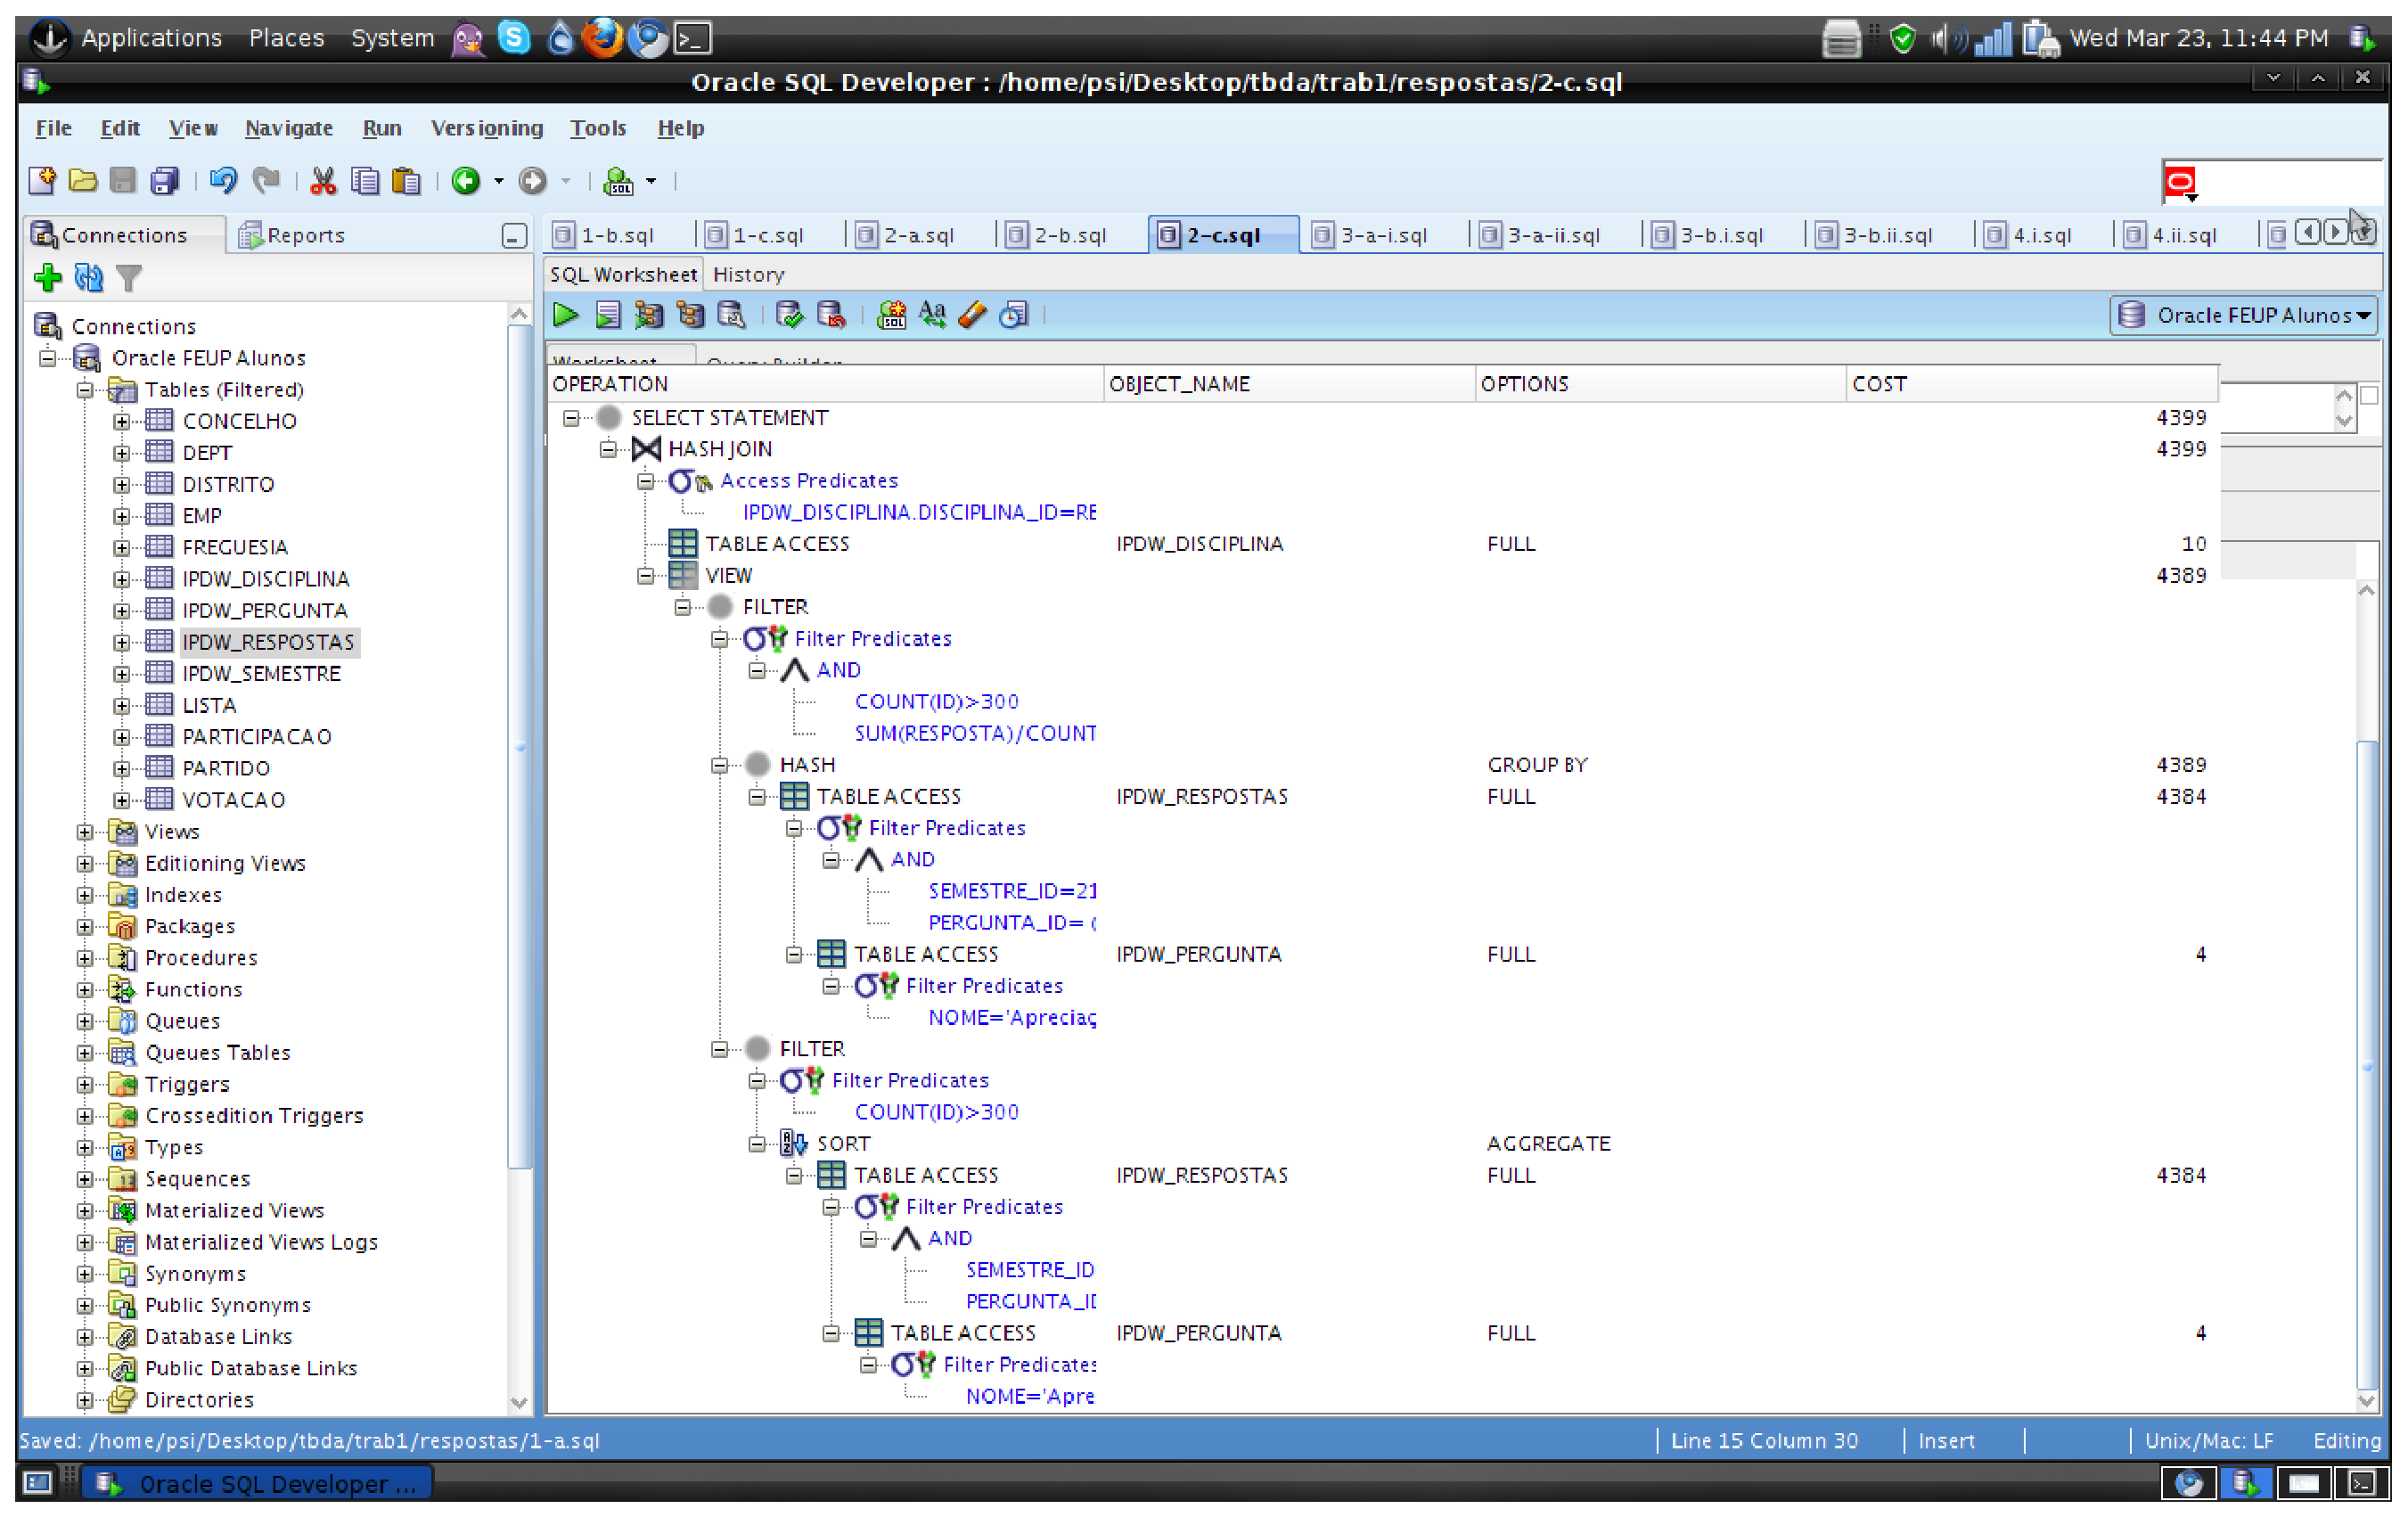
\includegraphics[width=1\textwidth]{2-c_B}}
   \end{center}
   \caption{Plano de execução para a Query \ref{sql:2-c}.}
\end{figure}

\begin{figure}[hpt]
   \begin{center}
      \ContinuedFloat
      \subfloat[Situação C]{\label{fig:plano_2-c_C}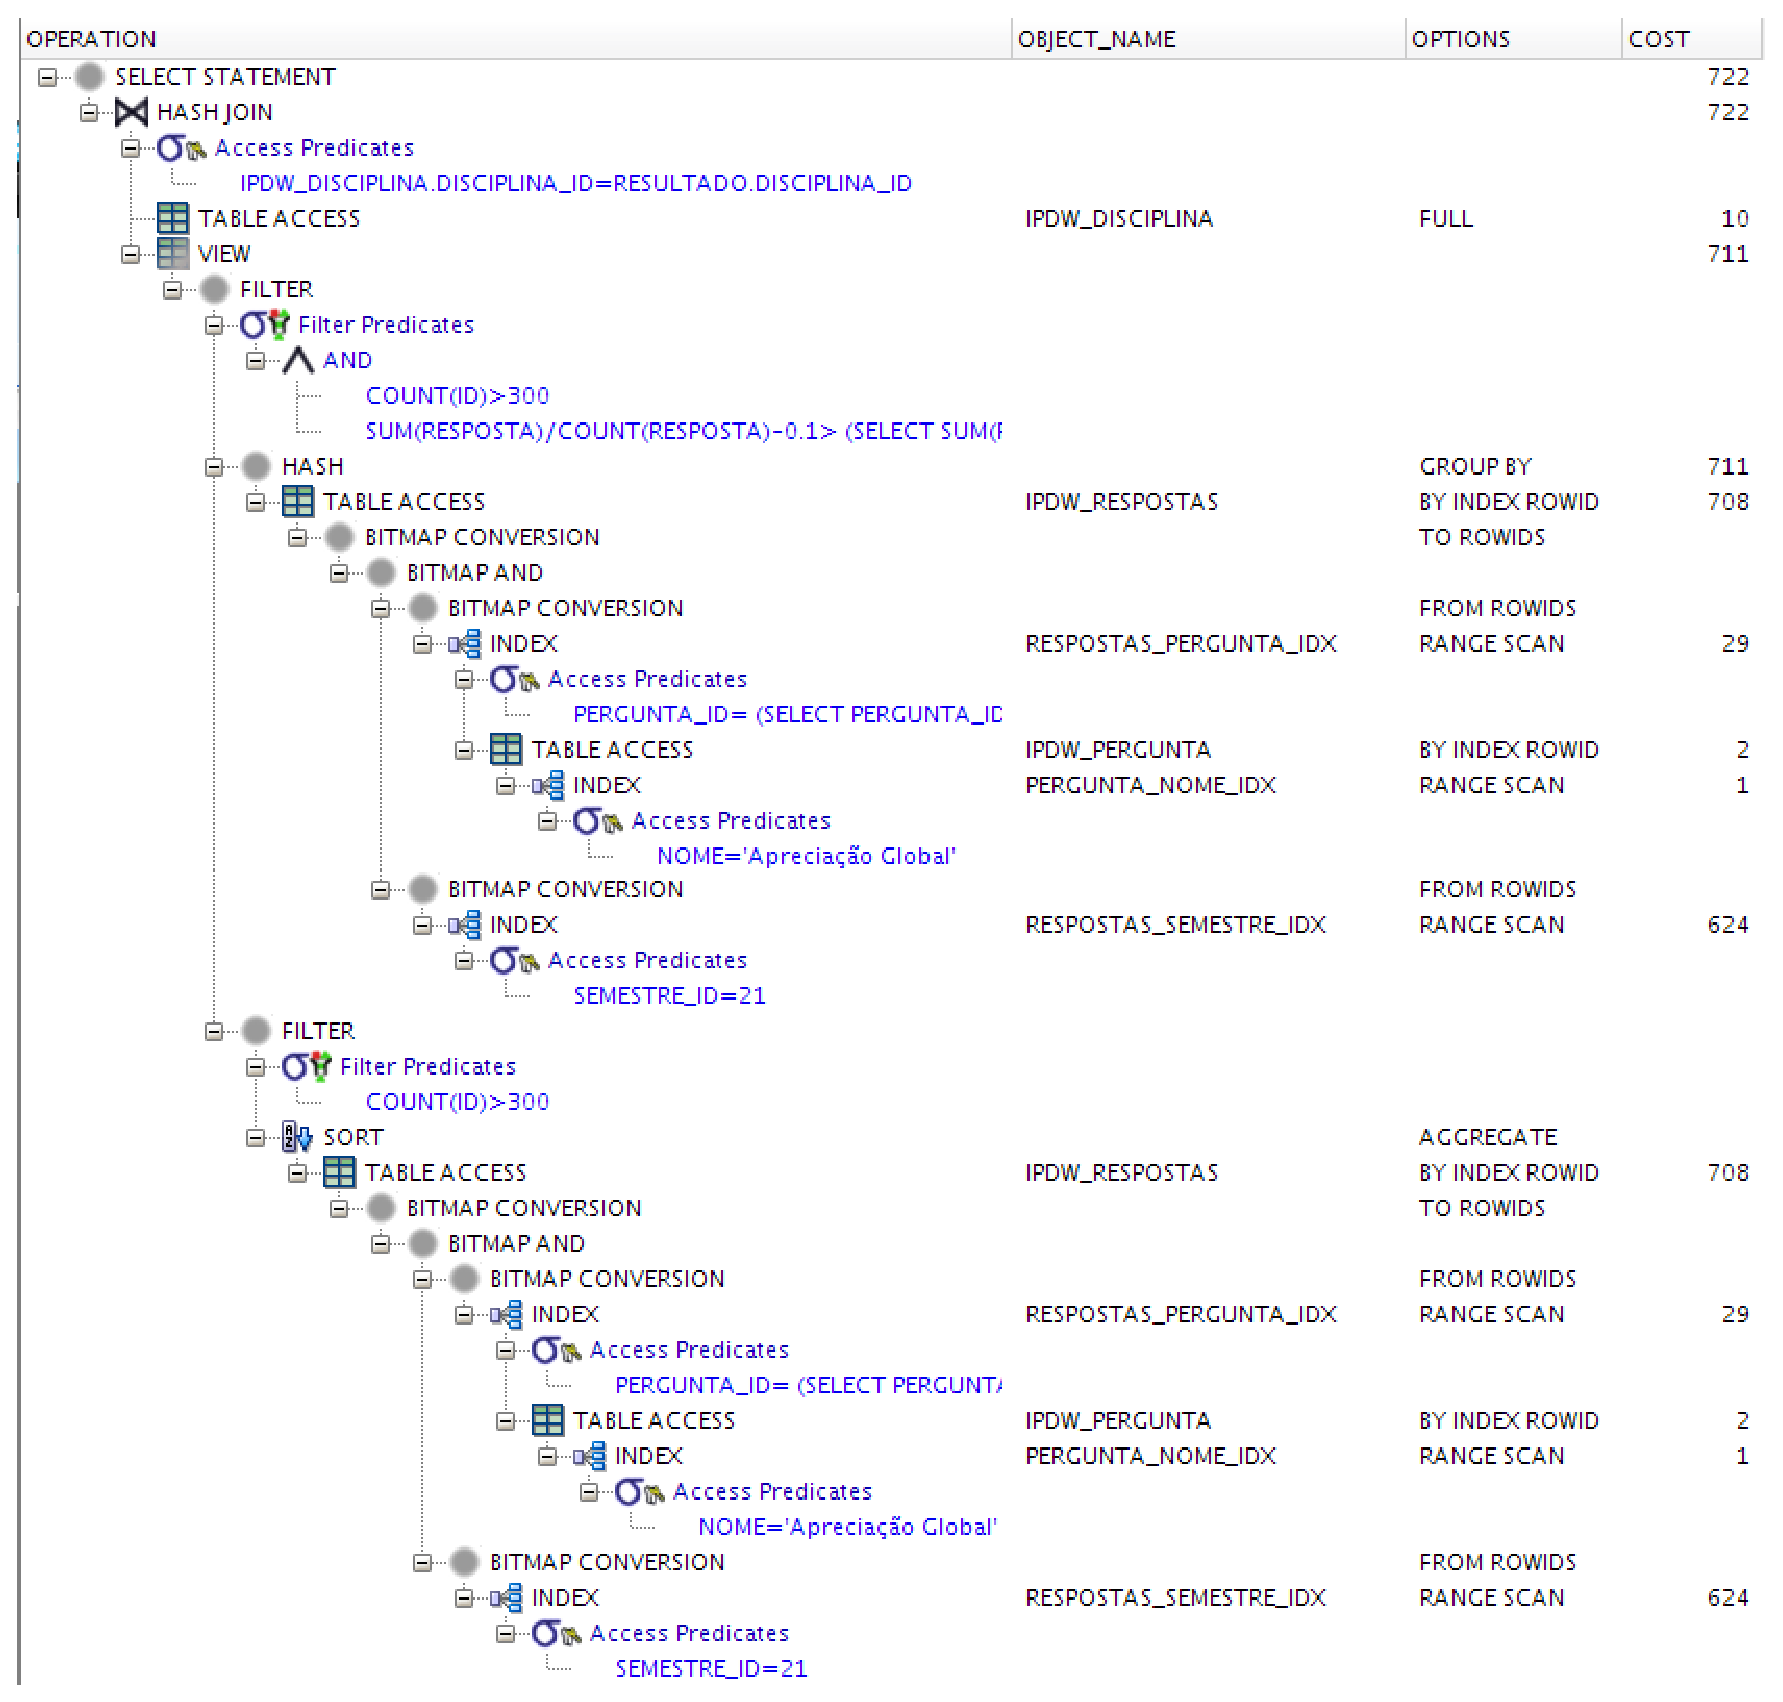
\includegraphics[width=1\textwidth]{2-c_C}}
   \end{center}
   \caption{Plano de execução para a Query \ref{sql:2-c}.}
\end{figure}

\begin{program}
   \verbatiminput{respostas/3-a-i.sql}
   \caption{Pergunta 3 baseada em ``not in'' com otimizador no modo CHOOSE.}
   \label{sql:3-a-i}
\end{program}

\begin{figure}[hpt]
   \begin{center}
      \subfloat[Situação A]{\label{fig:plano_3-a-i_A}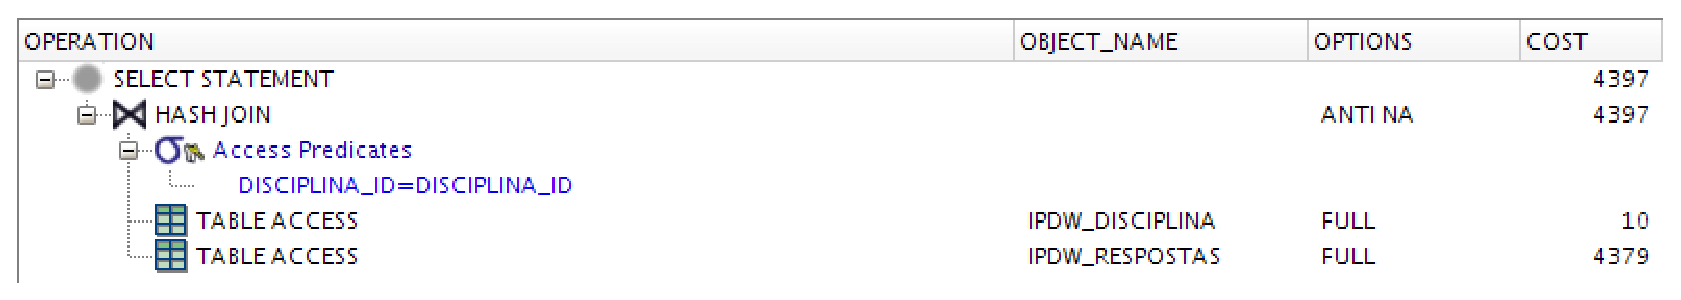
\includegraphics[width=1\textwidth]{3-a-i_A}}\\
      \subfloat[Situação B]{\label{fig:plano_3-a-i_B}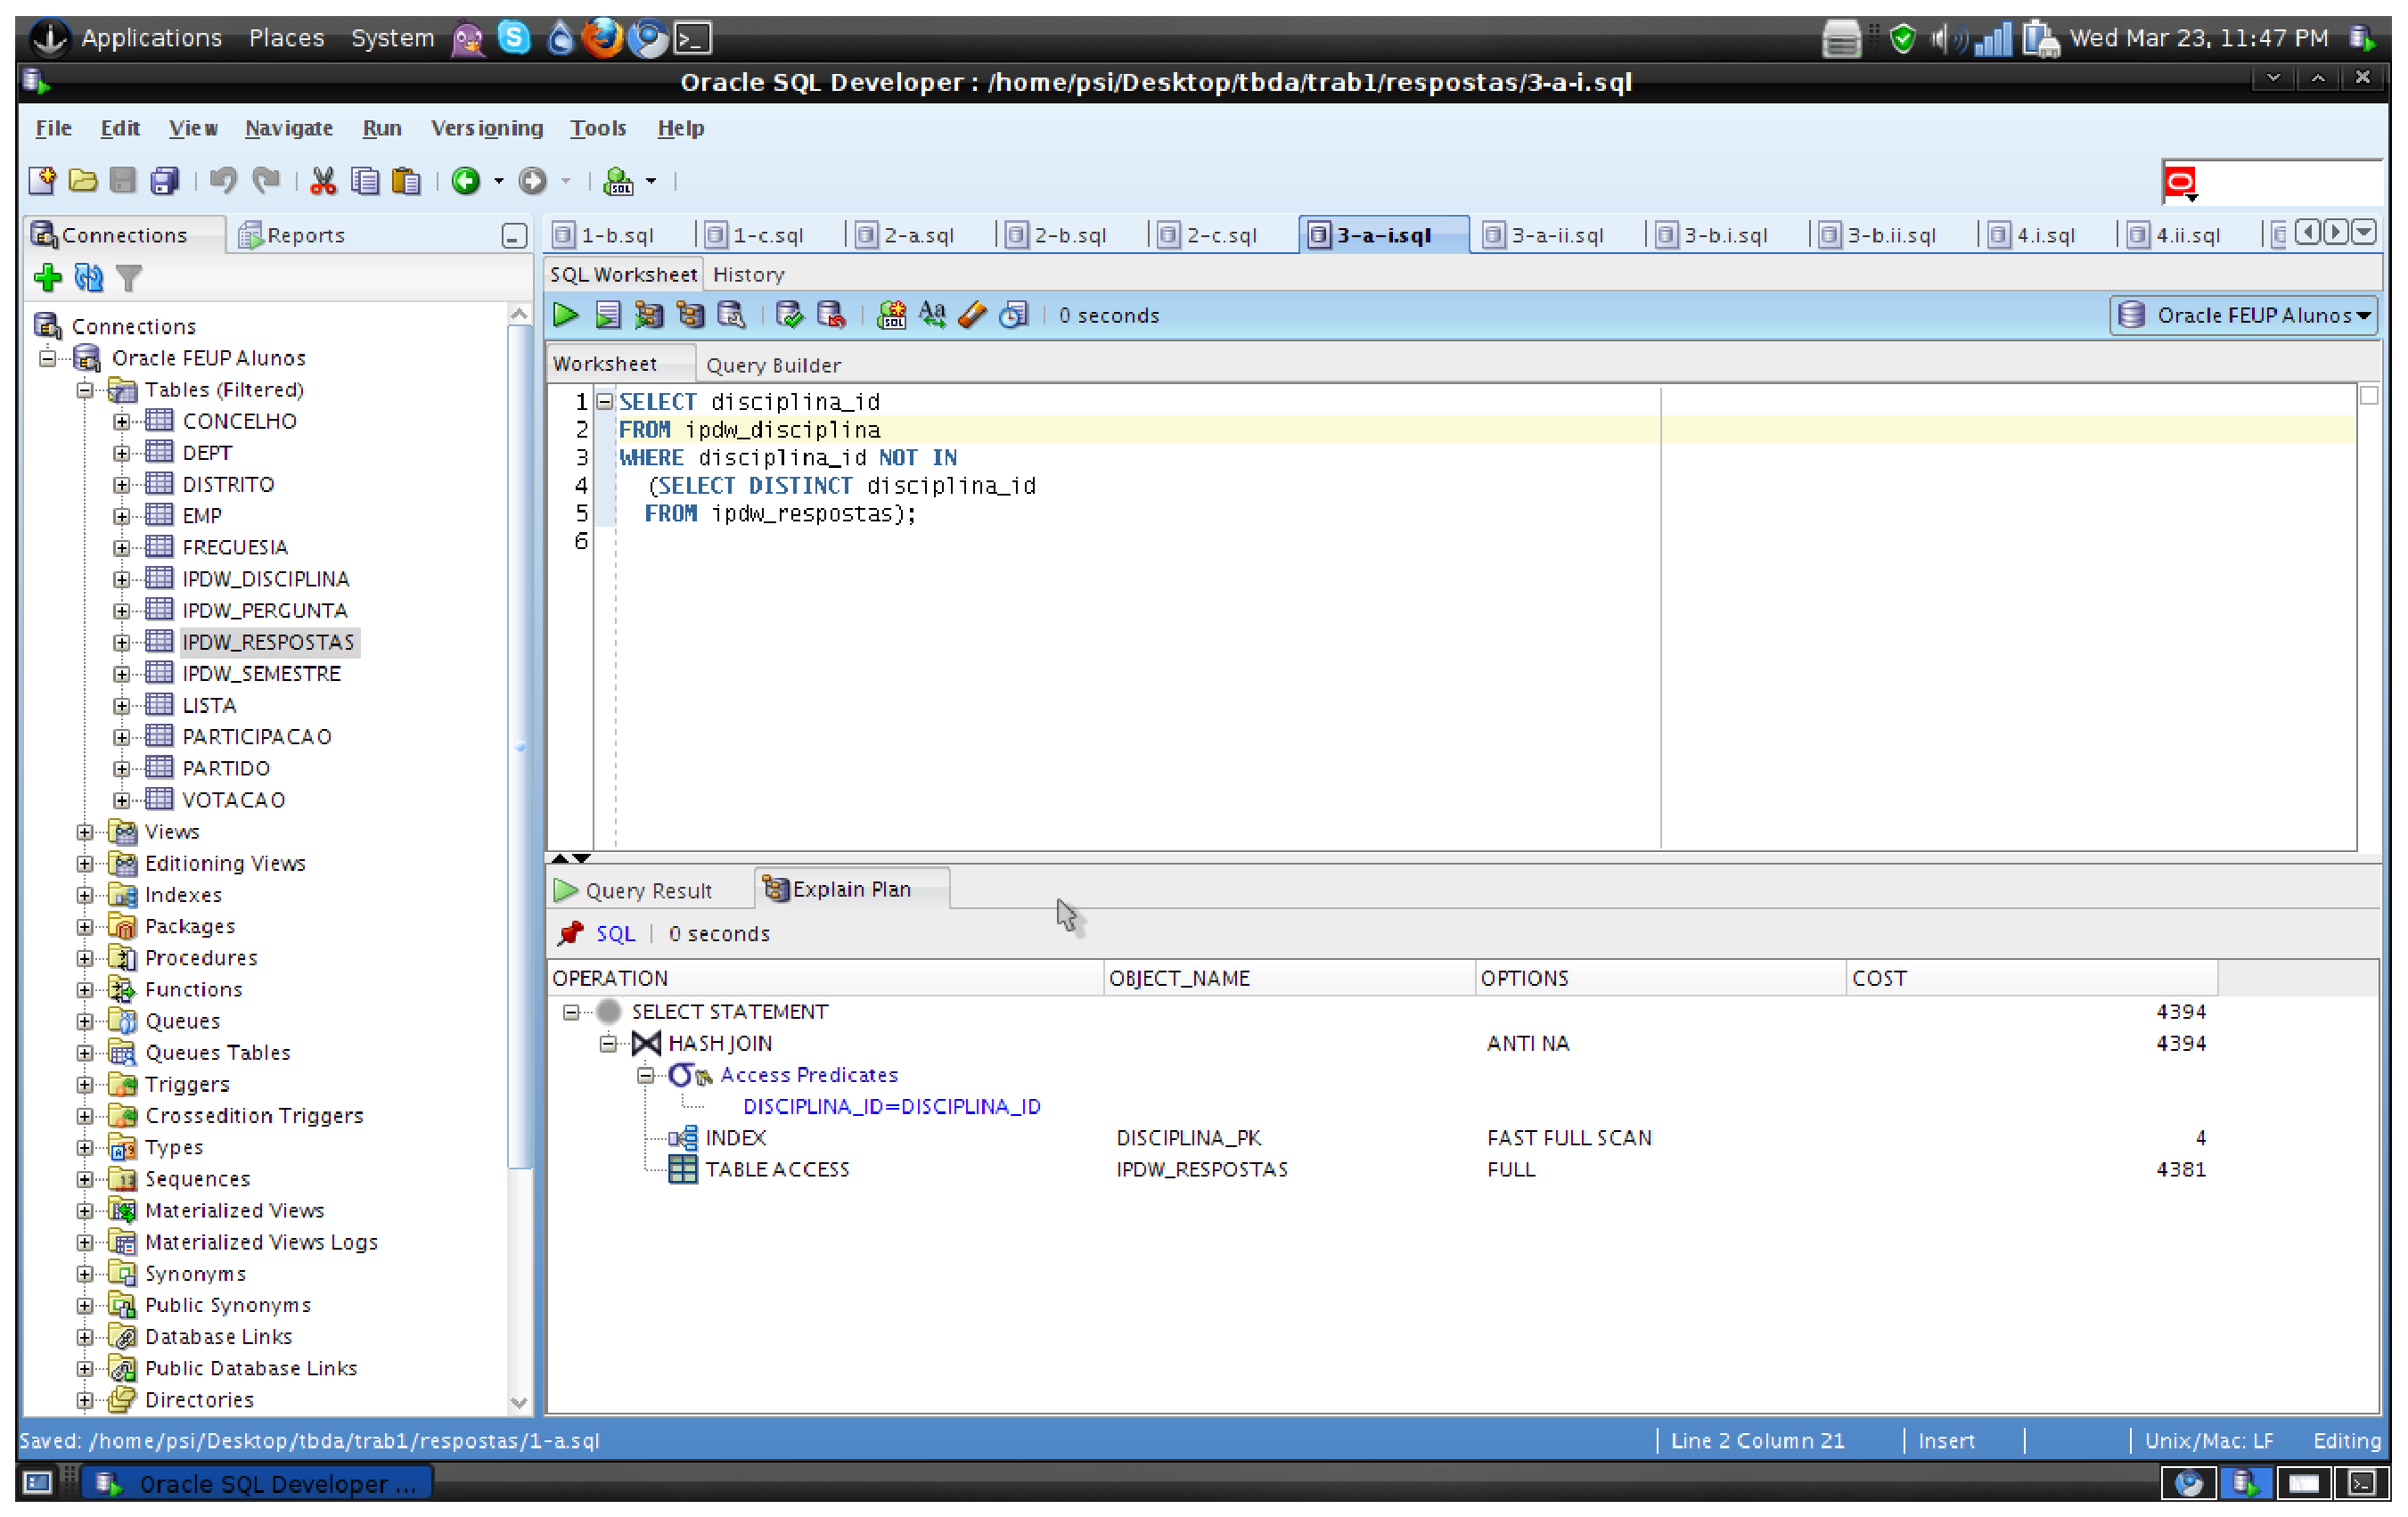
\includegraphics[width=1\textwidth]{3-a-i_B}}\\
      \subfloat[Situação C]{\label{fig:plano_3-a-i_C}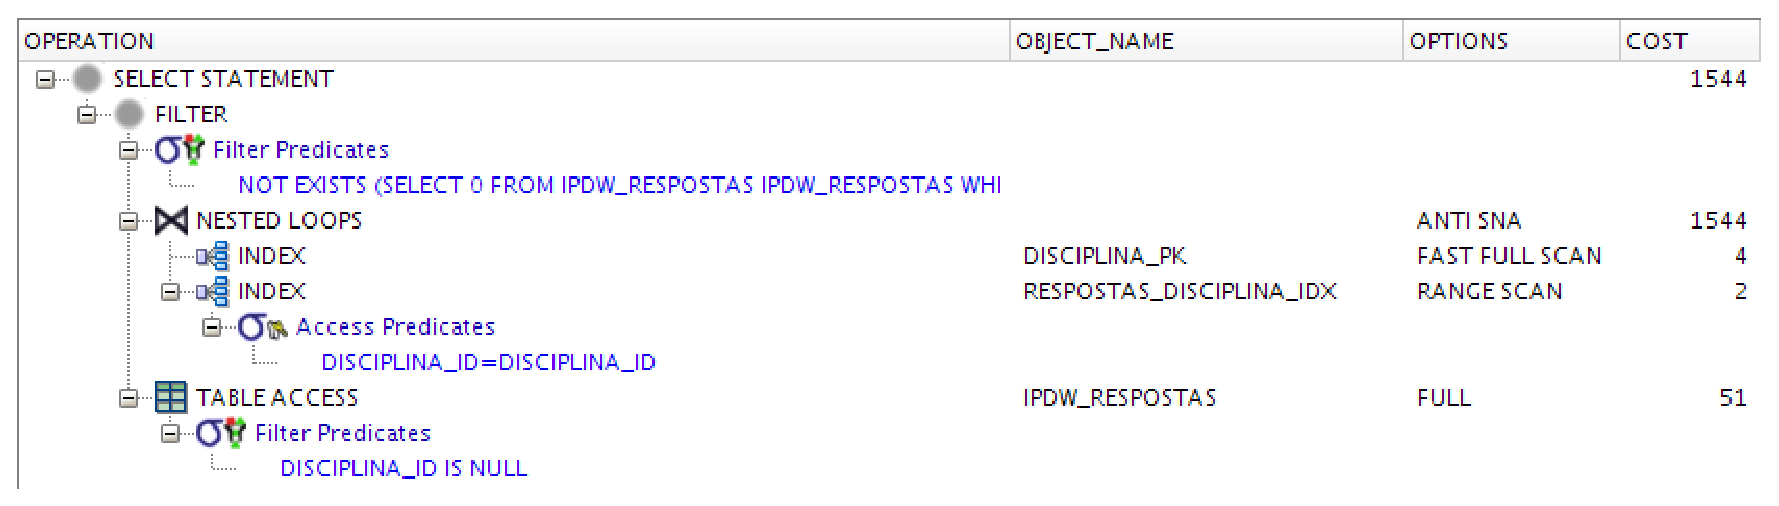
\includegraphics[width=1\textwidth]{3-a-i_C}}
   \end{center}
   \caption{Plano de execução para a Query \ref{sql:3-a-i}.}
   \label{fig:plano_3-a-i}
\end{figure}

\begin{program}
   \verbatiminput{respostas/3-a-ii.sql}
   \caption{Pergunta 3 baseada em ``not in'' com otimizador no modo RULE.}
   \label{sql:3-a-ii}
\end{program}

\begin{figure}[hpt]
   \begin{center}
      \subfloat[Situação A]{\label{fig:plano_3-a-ii_A}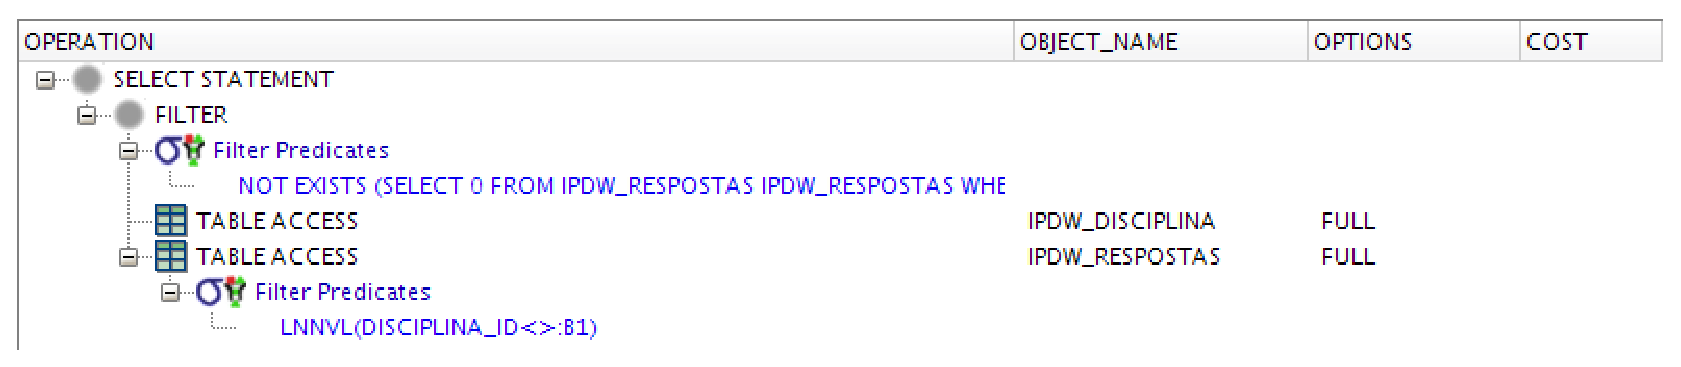
\includegraphics[width=1\textwidth]{3-a-ii_A}}\\
      \subfloat[Situação B]{\label{fig:plano_3-a-ii_B}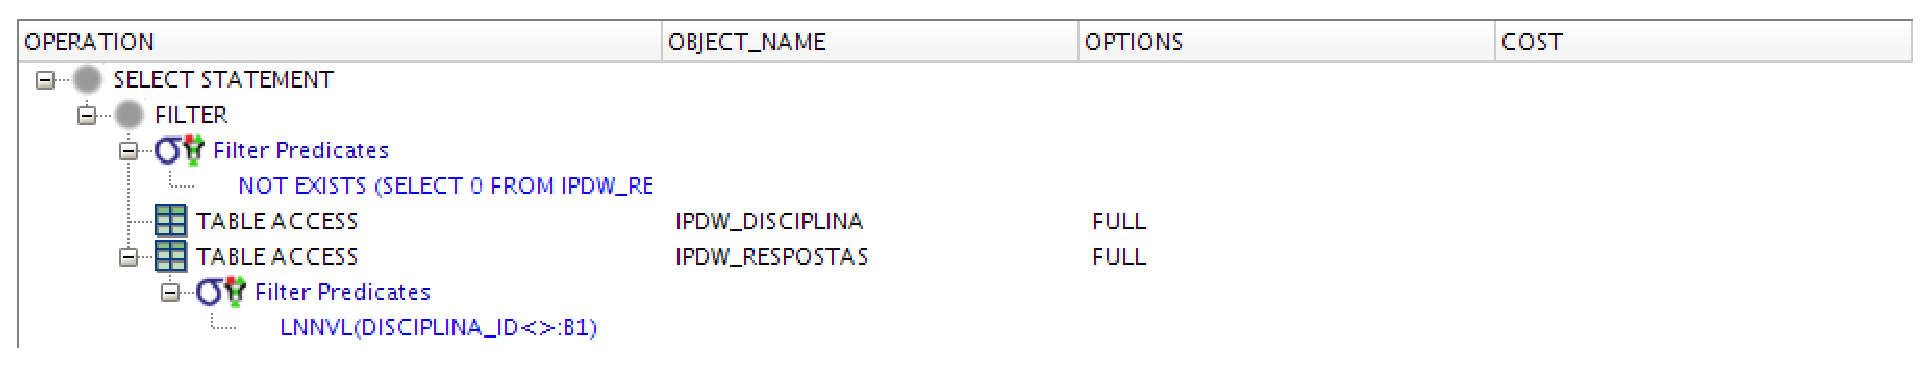
\includegraphics[width=1\textwidth]{3-a-ii_B}}\\
      \subfloat[Situação C]{\label{fig:plano_3-a-ii_C}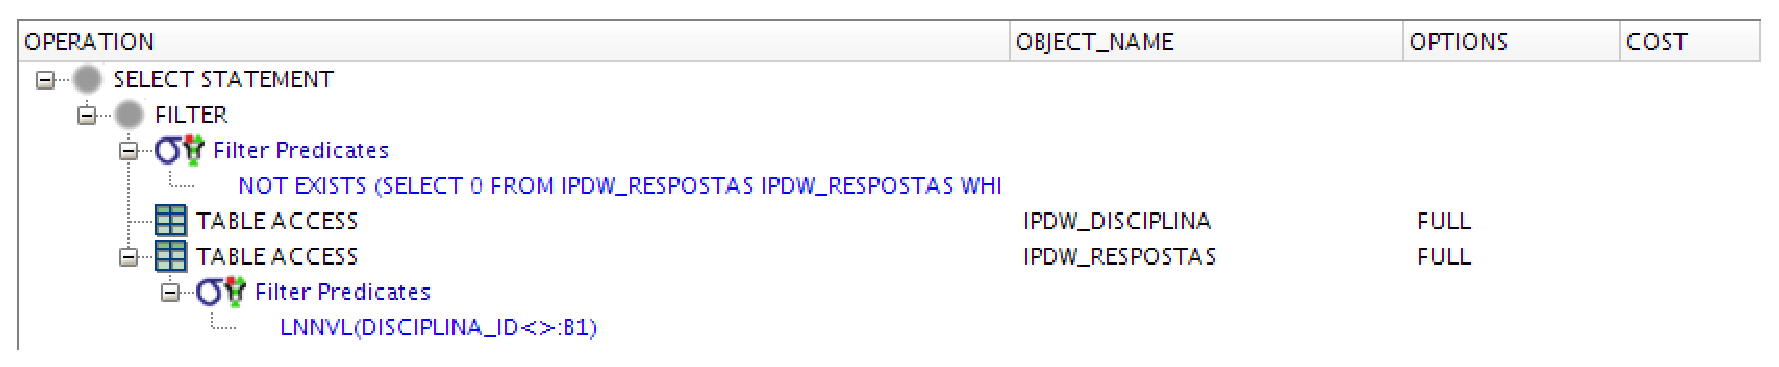
\includegraphics[width=1\textwidth]{3-a-ii_C}}
   \end{center}
   \caption{Plano de execução para a Query \ref{sql:3-a-ii}.}
   \label{fig:plano_3-a-ii}
\end{figure}

\begin{program}
   \verbatiminput{respostas/3-b.i.sql}
   \caption{Pergunta 3 baseada em junção externa e filtragem para nulo com otimizador no modo CHOOSE.}
   \label{sql:3-b-i}
\end{program}

\begin{figure}[hpt]
   \begin{center}
      \subfloat[Situação A]{\label{fig:plano_3-b-i_A}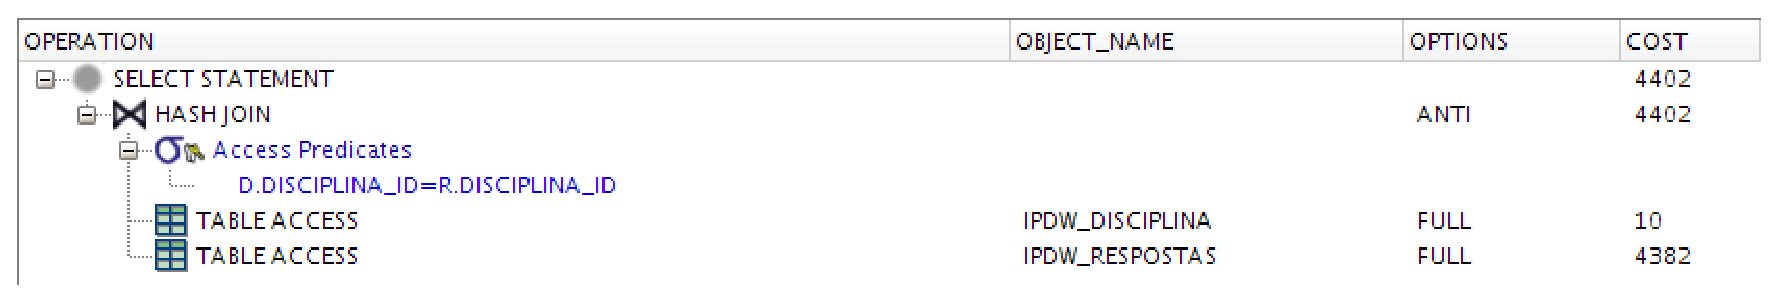
\includegraphics[width=1\textwidth]{3-b-i_A}}\\ 
      \subfloat[Situação B]{\label{fig:plano_3-b-i_B}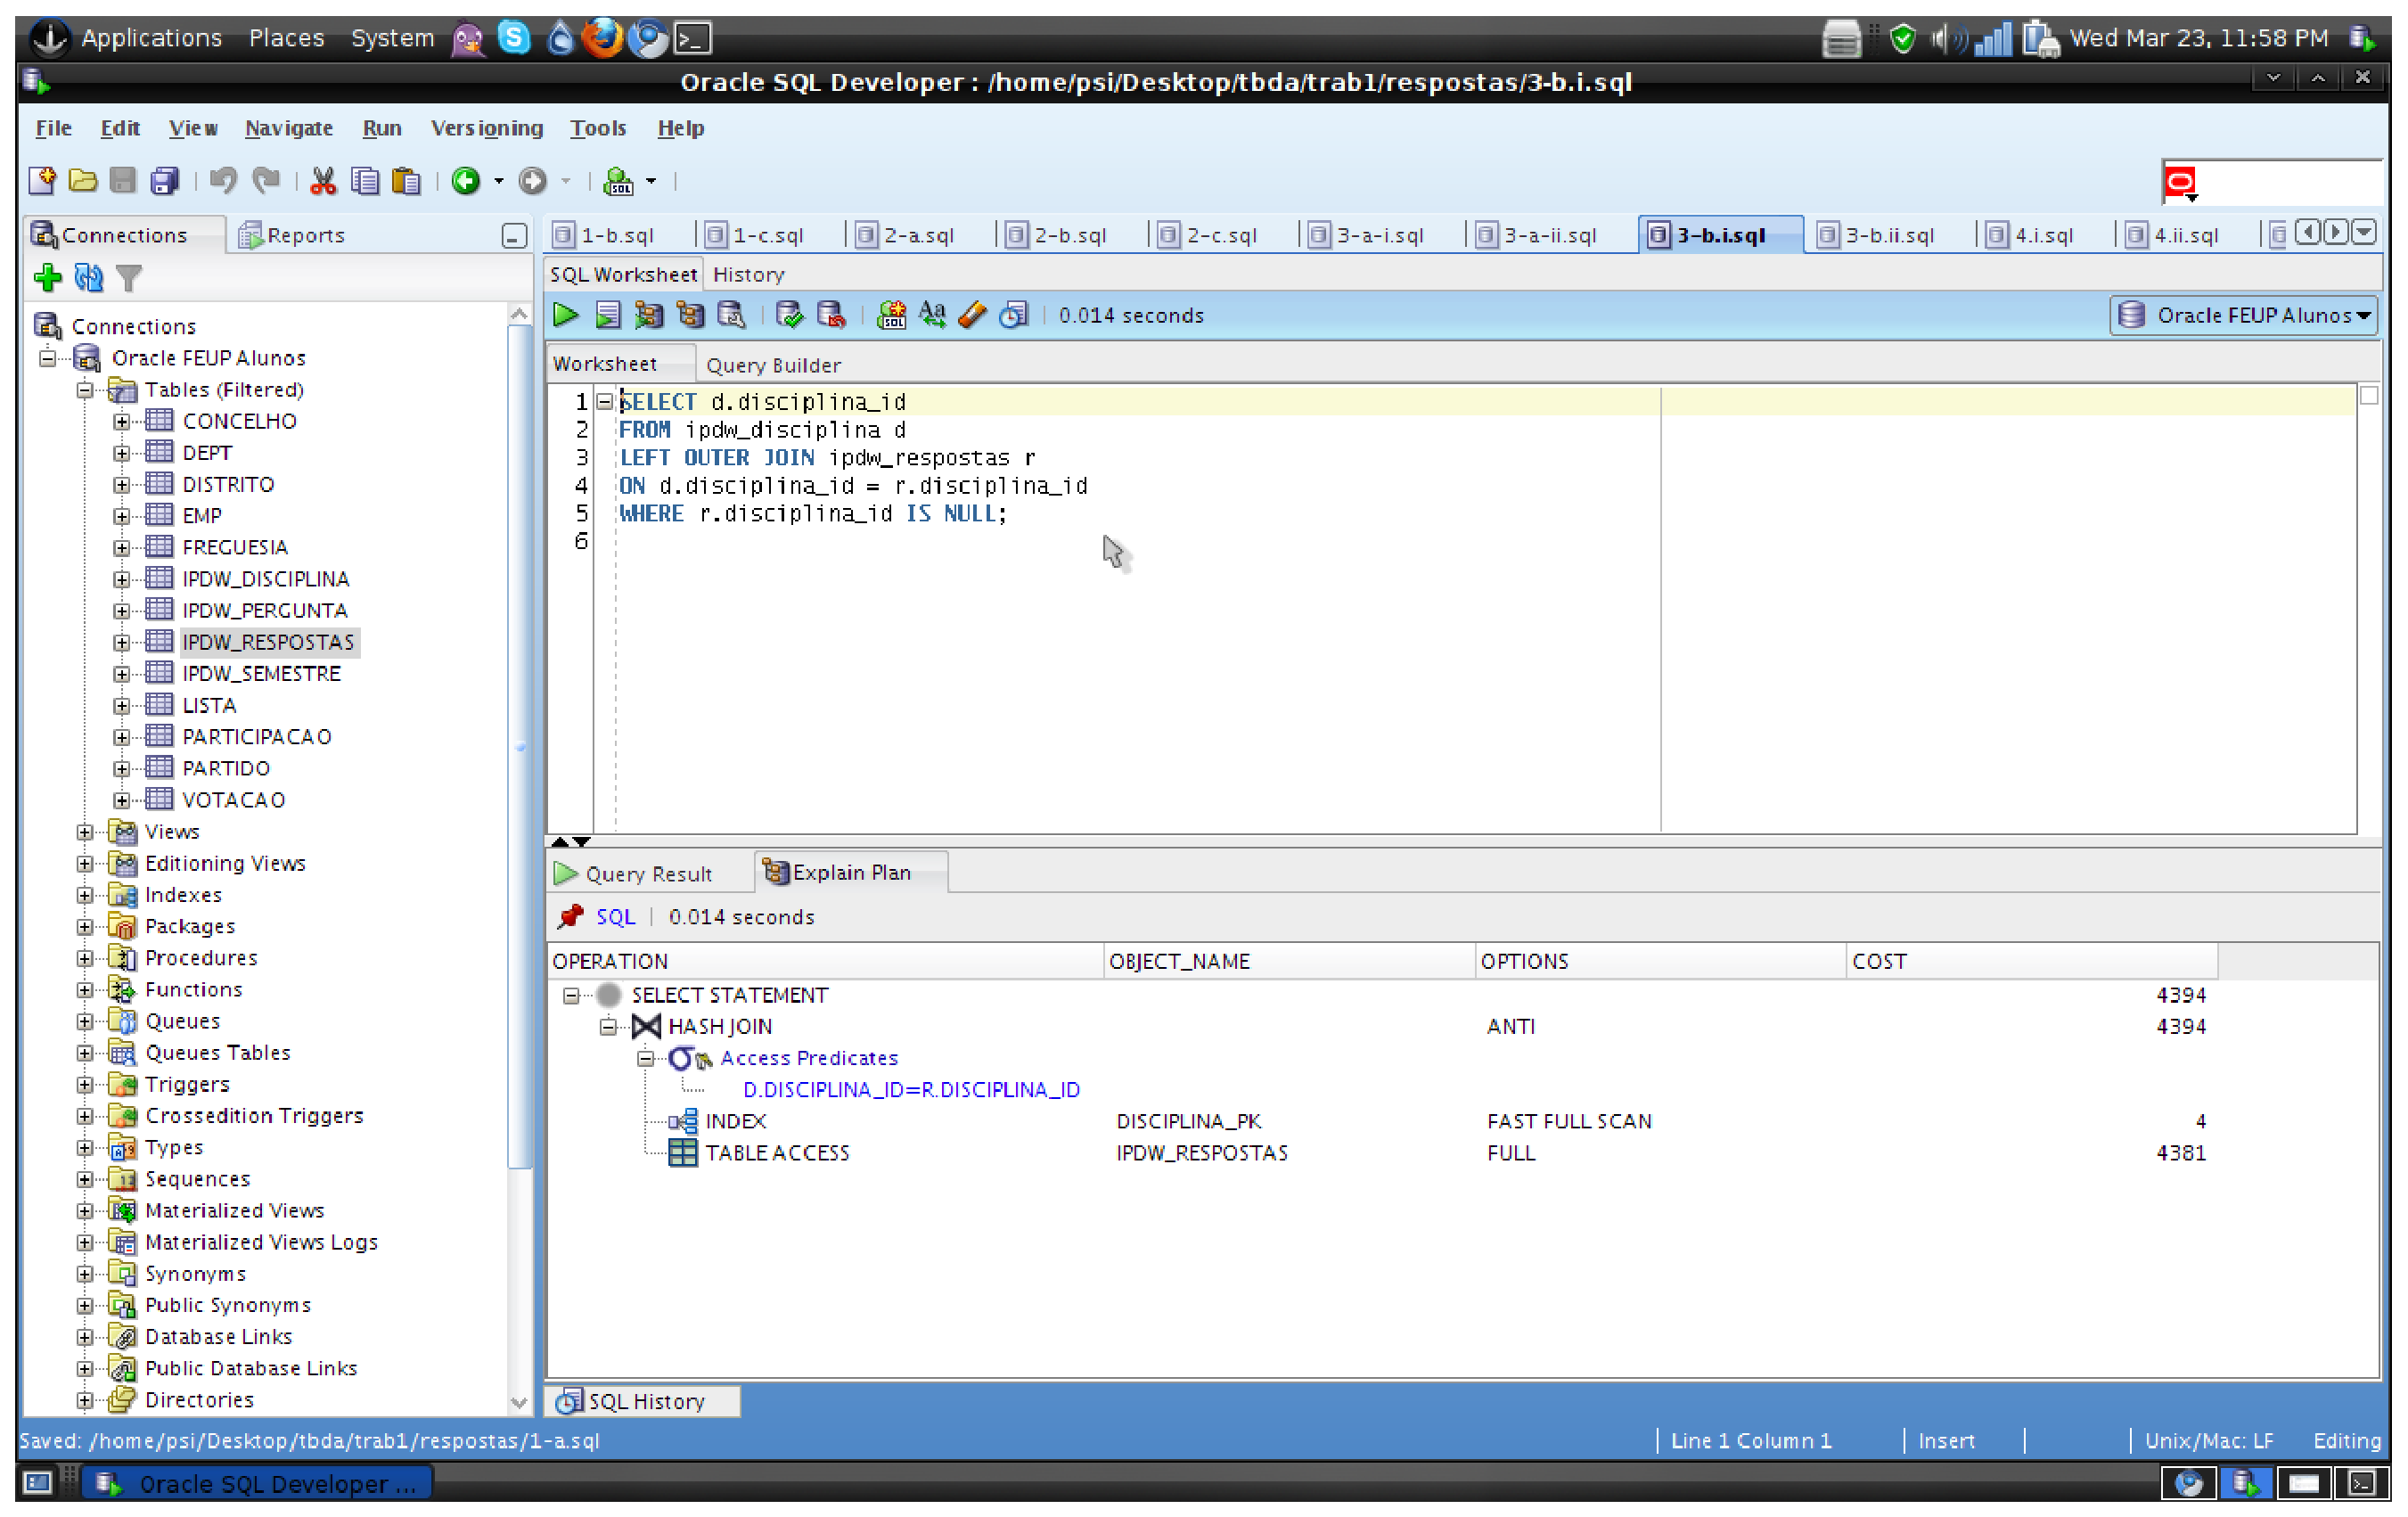
\includegraphics[width=1\textwidth]{3-b-i_B}}\\
      \subfloat[Situação C]{\label{fig:plano_3-b-i_C}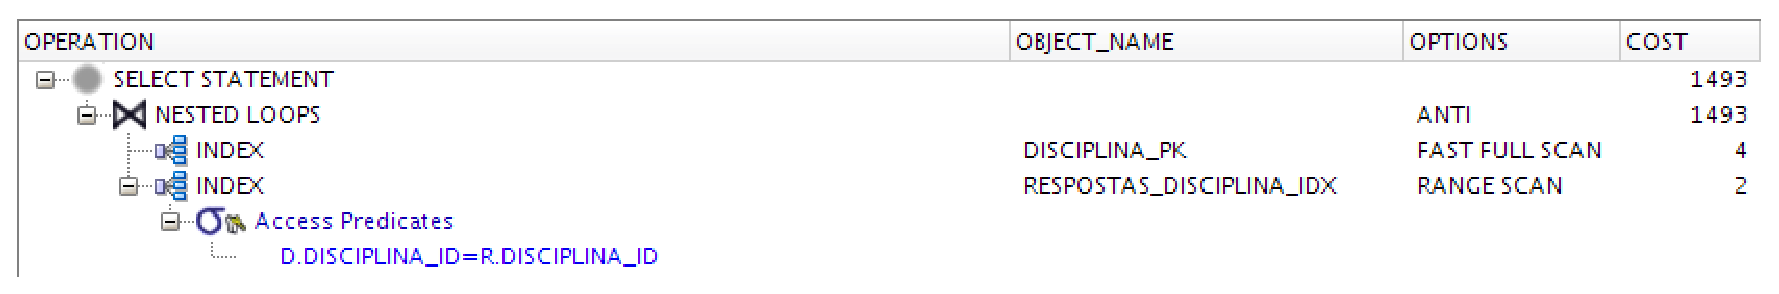
\includegraphics[width=1\textwidth]{3-b-i_C}}
   \end{center}
   \caption{Plano de execução para a Query \ref{sql:3-b-i}.}
   \label{fig:plano_3-b-i}
\end{figure}

\begin{program}
   \verbatiminput{respostas/3-b.ii.sql}
   \caption{Pergunta 3 baseada em junção externa e filtragem para nulo com otimizador no modo RULE.}
   \label{sql:3-b-ii}
\end{program}

\begin{figure}[hpt]
   \begin{center}
      \subfloat[Situação A]{\label{fig:plano_3-b-ii_A}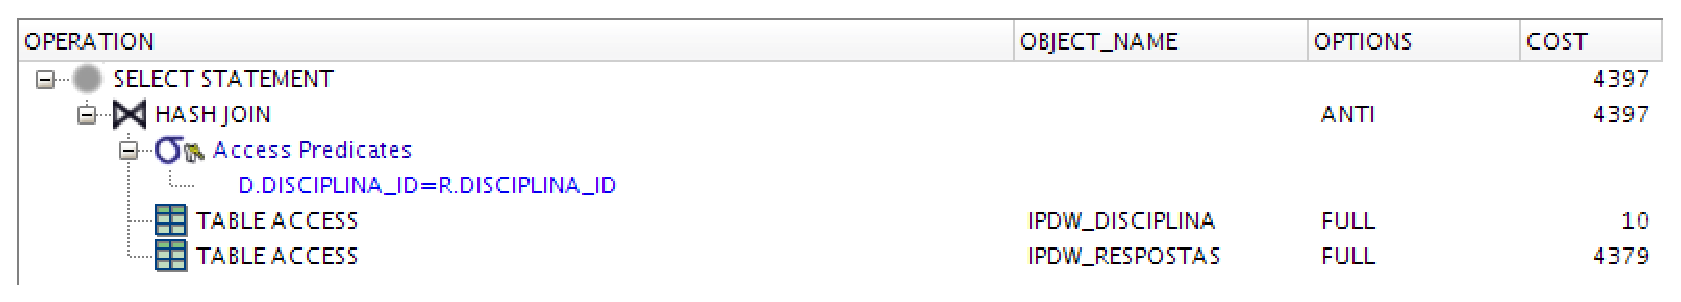
\includegraphics[width=1\textwidth]{3-b-ii_A}}\\
      \subfloat[Situação B]{\label{fig:plano_3-b-ii_B}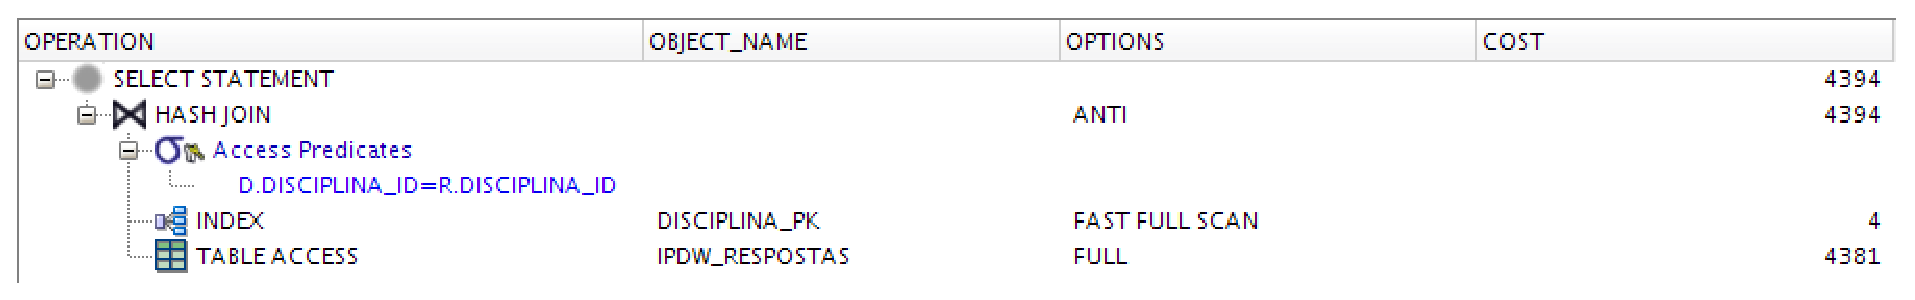
\includegraphics[width=1\textwidth]{3-b-ii_B}}\\
      \subfloat[Situação C]{\label{fig:plano_3-b-ii_C}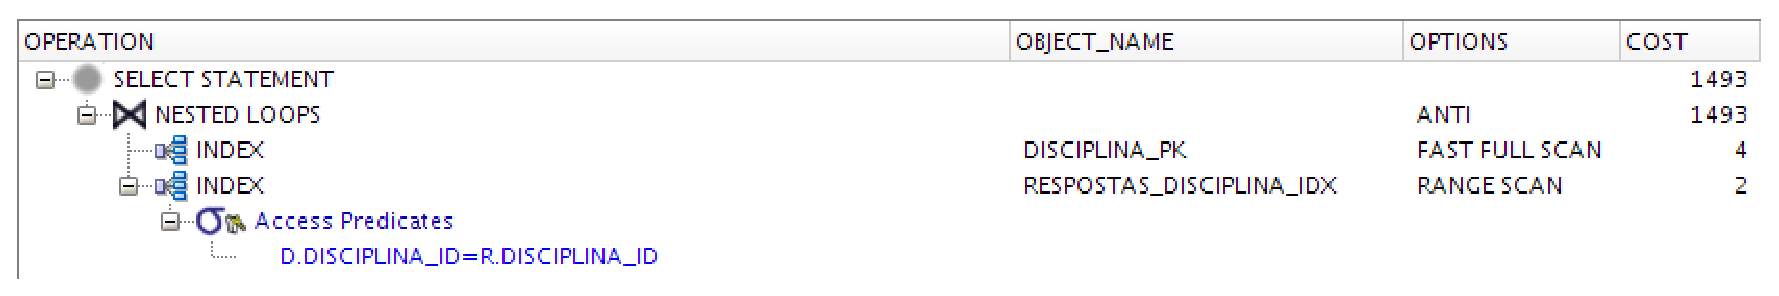
\includegraphics[width=1\textwidth]{3-b-ii_C}}
   \end{center}
   \caption{Plano de execução para a Query \ref{sql:3-b-ii}.}
   \label{fig:plano_3-b-ii}
\end{figure}

\begin{program}
   \verbatiminput{respostas/4.i.sql}
   \caption{Pergunta 4 utilizando o método da dupla negação.}
   \label{sql:4-i}
\end{program}

\begin{figure}[hpt]
   \begin{center}
      \subfloat[Situação A]{\label{fig:plano_4-i_A}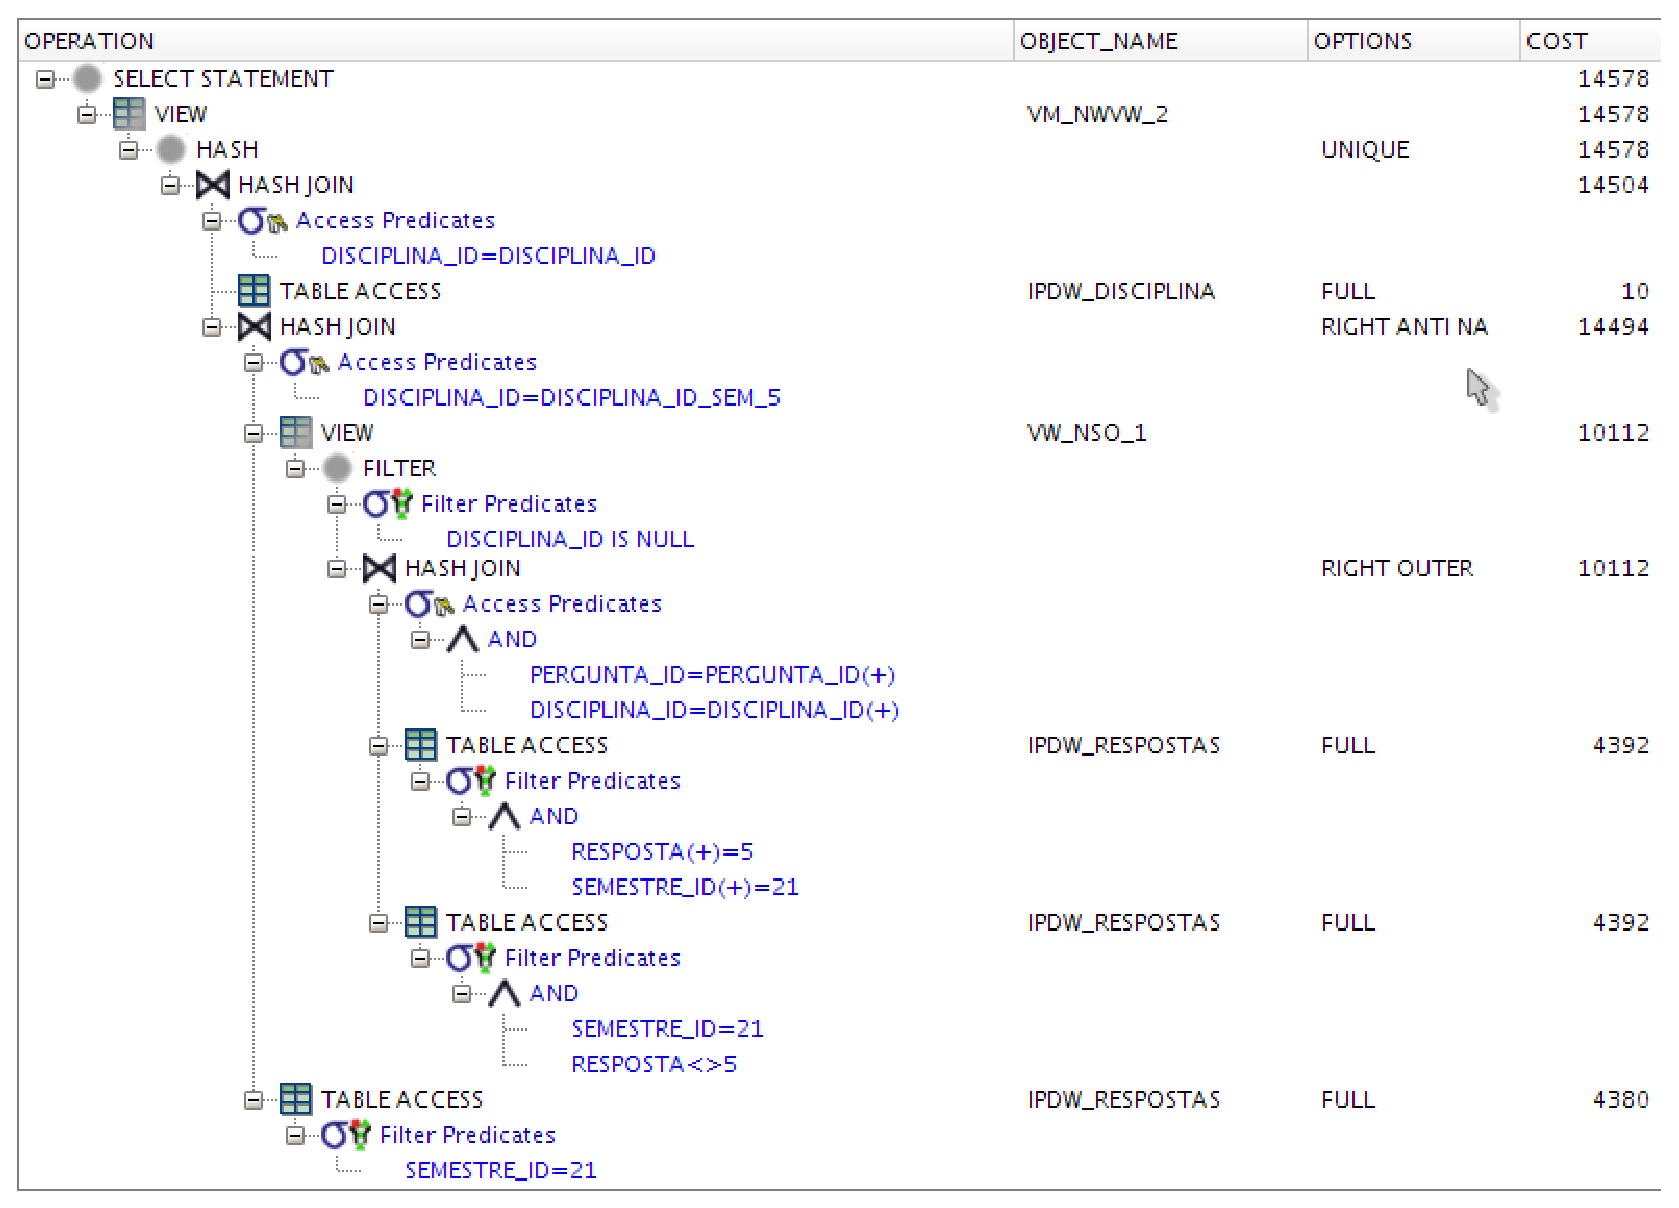
\includegraphics[width=1\textwidth]{4-i_A}}\\
   \end{center}
   \caption{Plano de execução para a Query \ref{sql:4-i}.}
   \label{fig:plano_4-i}
\end{figure}

\begin{figure}[hpt]
   \ContinuedFloat
   \begin{center}
      \subfloat[Situação B]{\label{fig:plano_4-i_B}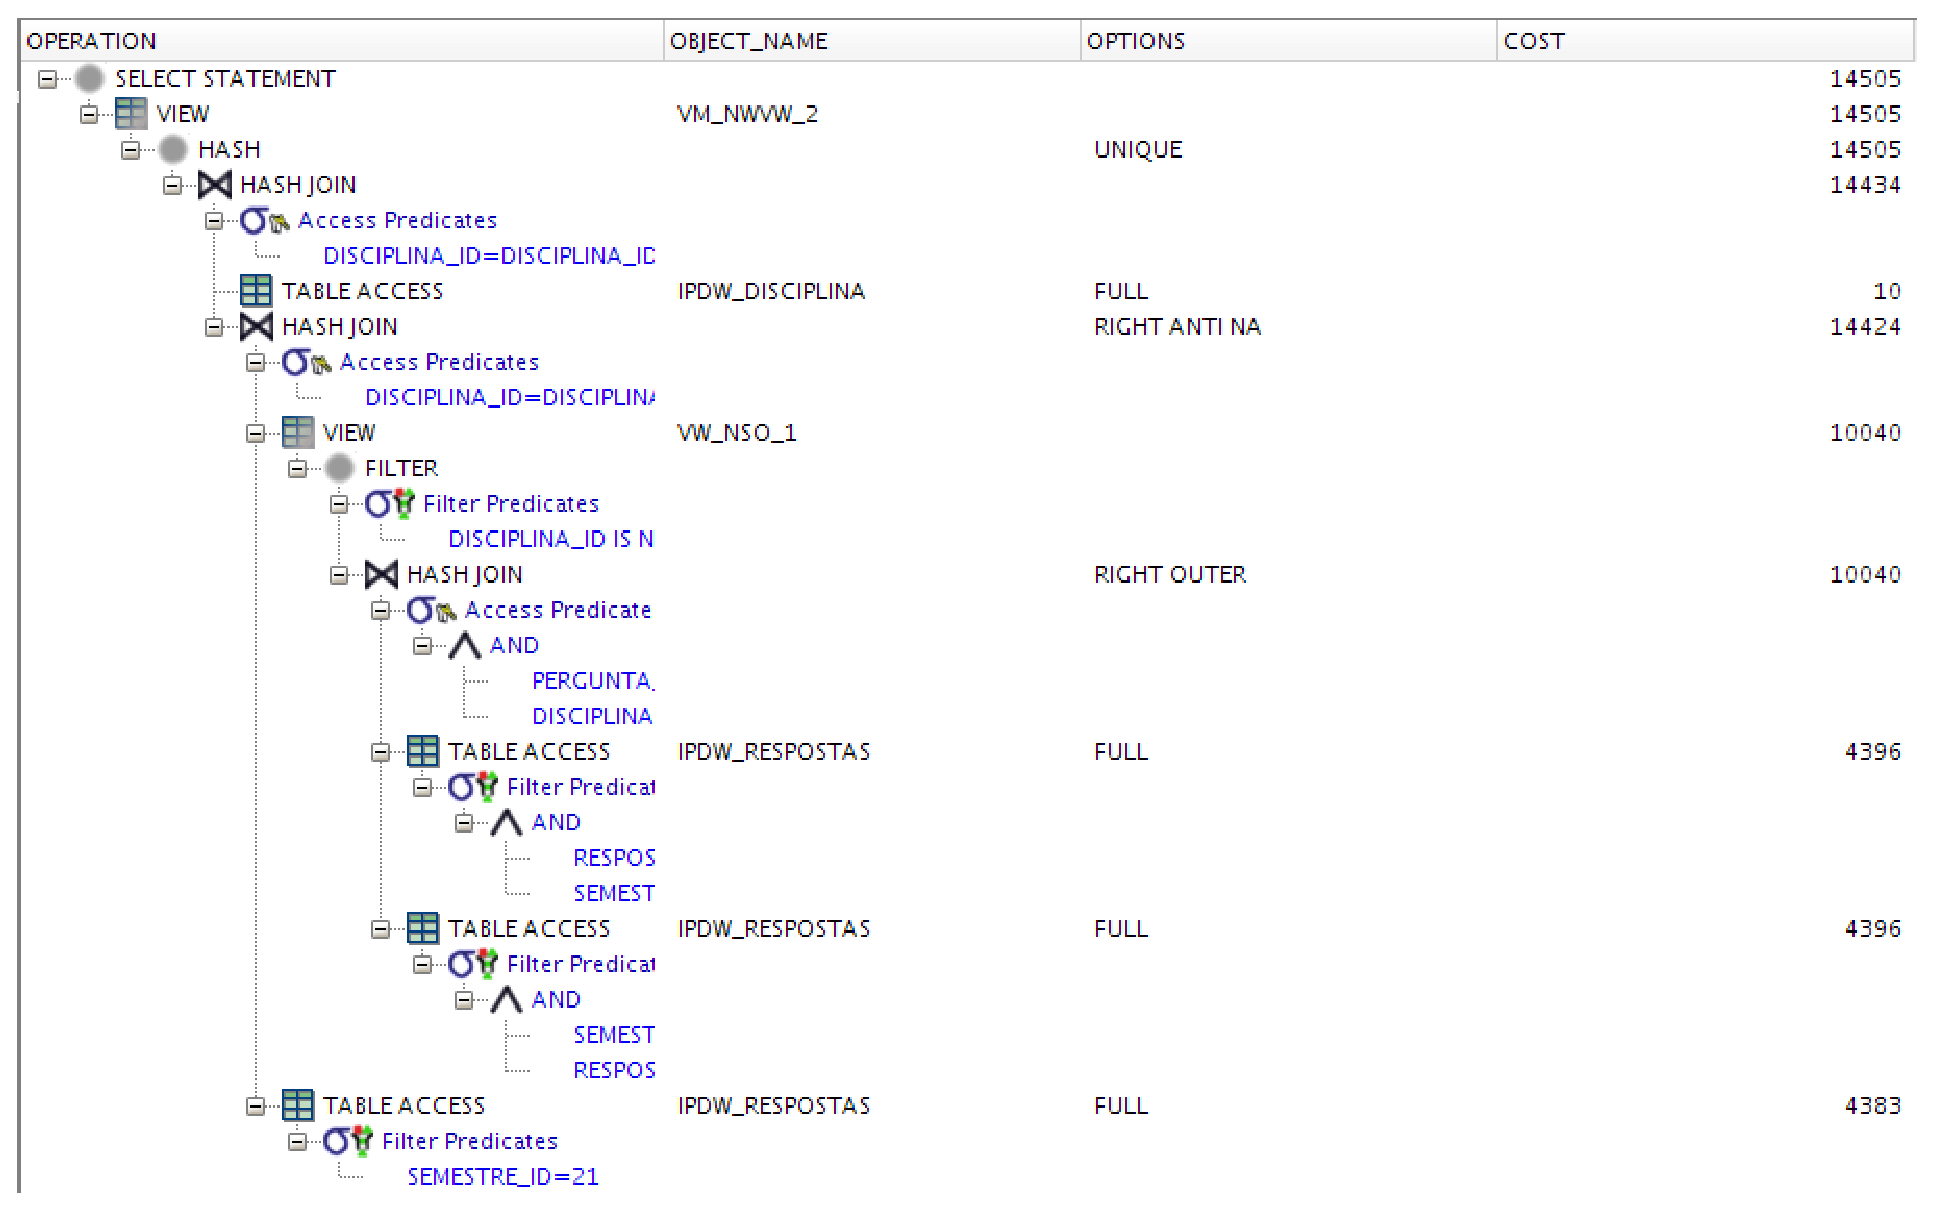
\includegraphics[width=1\textwidth]{4-i_B}}\\
   \end{center}
   \caption{Plano de execução para a Query \ref{sql:4-i}.}
\end{figure}

\begin{figure}[hpt]
   \ContinuedFloat
   \begin{center}
      \subfloat[Situação C]{\label{fig:plano_4-i_C}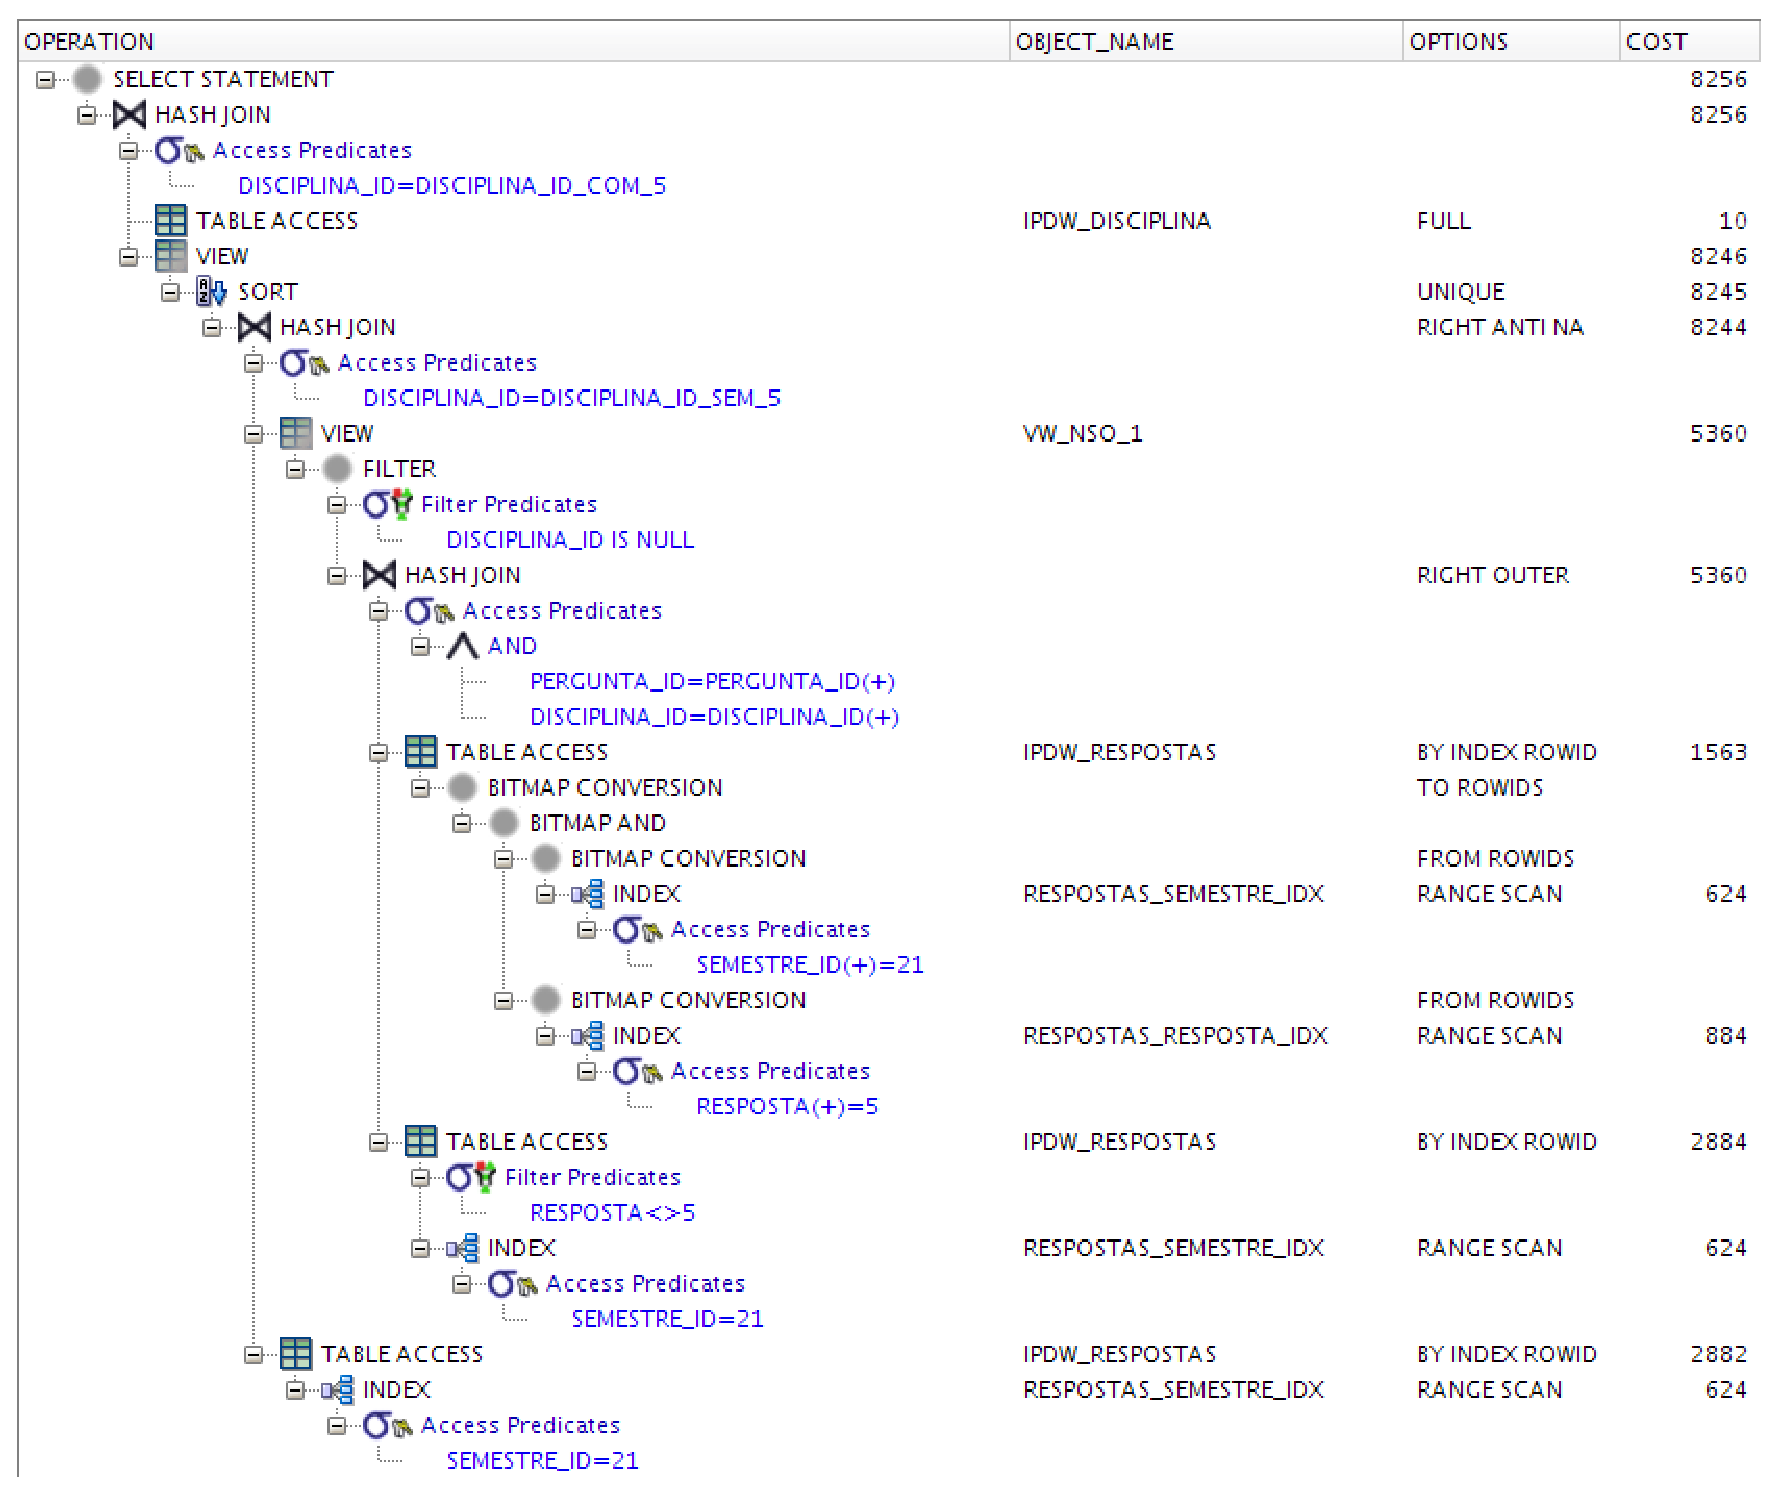
\includegraphics[width=1\textwidth]{4-i_C}}
   \end{center}
   \caption{Plano de execução para a Query \ref{sql:4-i}.}
\end{figure}

\begin{program}
   \verbatiminput{respostas/4.ii.sql}
   \caption{Pergunta 4 utilizando o método da contagem.}
   \label{sql:4-ii}
\end{program}

\begin{figure}[hpt]
   \begin{center}
      \subfloat[Situação A]{\label{fig:plano_4-ii_A}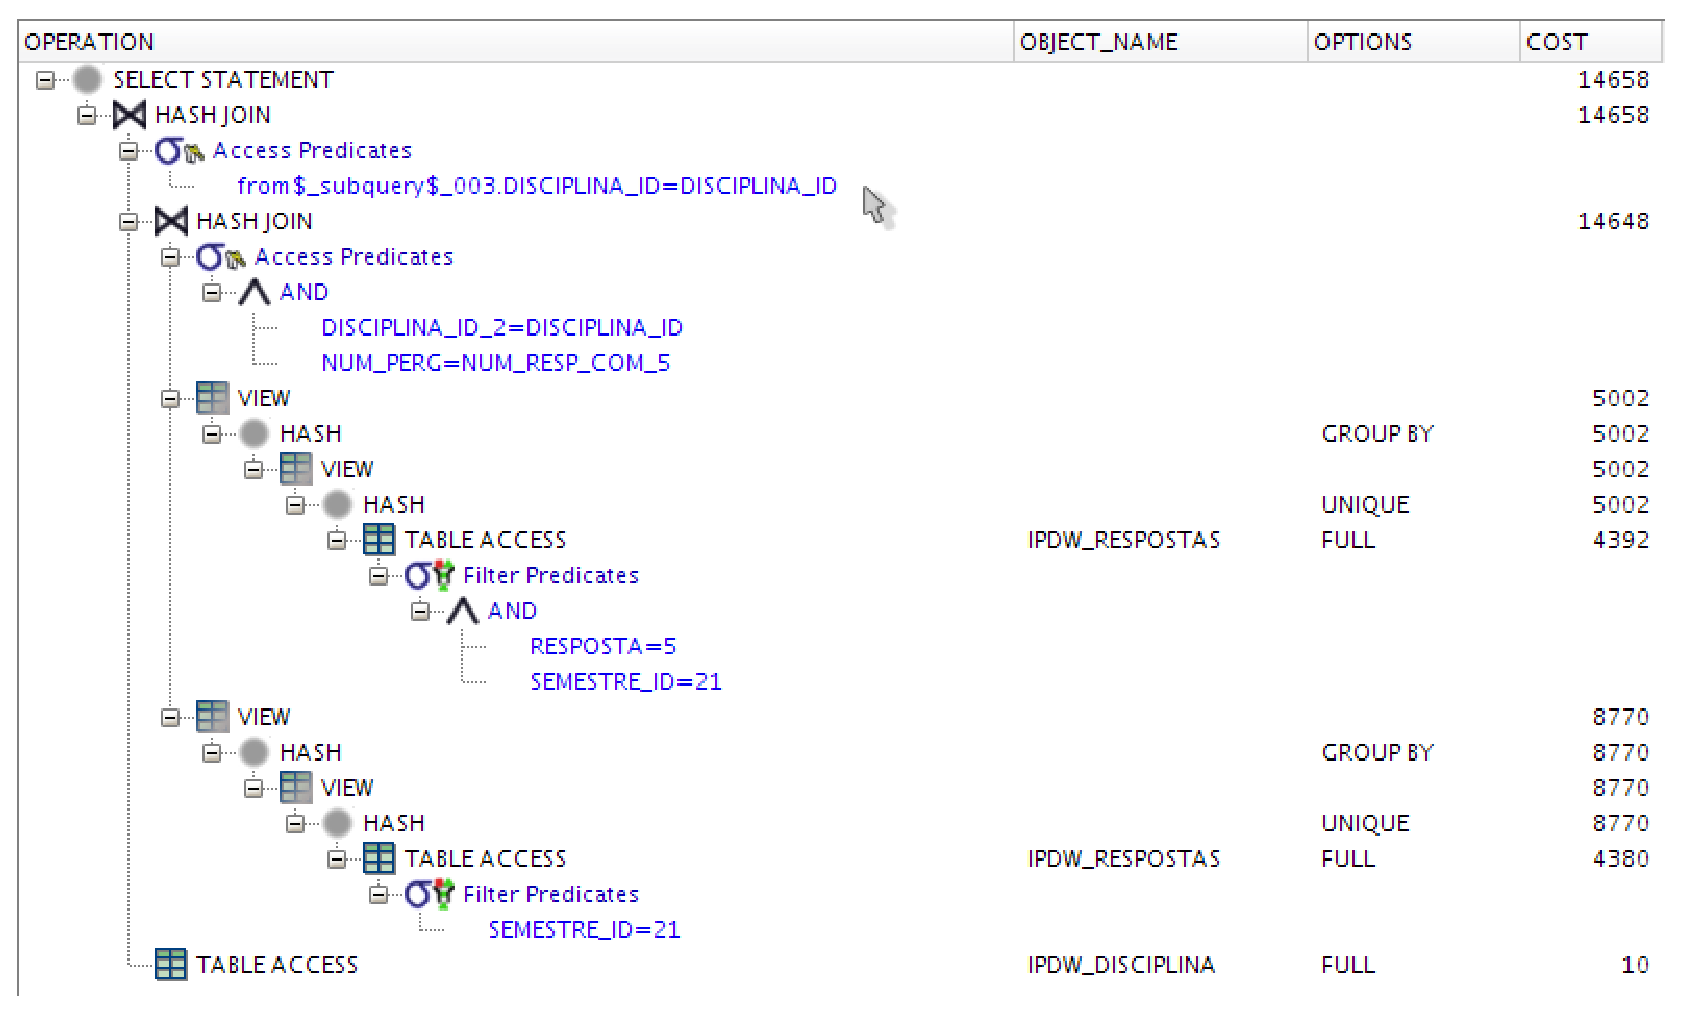
\includegraphics[width=1\textwidth]{4-ii_A}}\\
      \subfloat[Situação B]{\label{fig:plano_4-ii_B}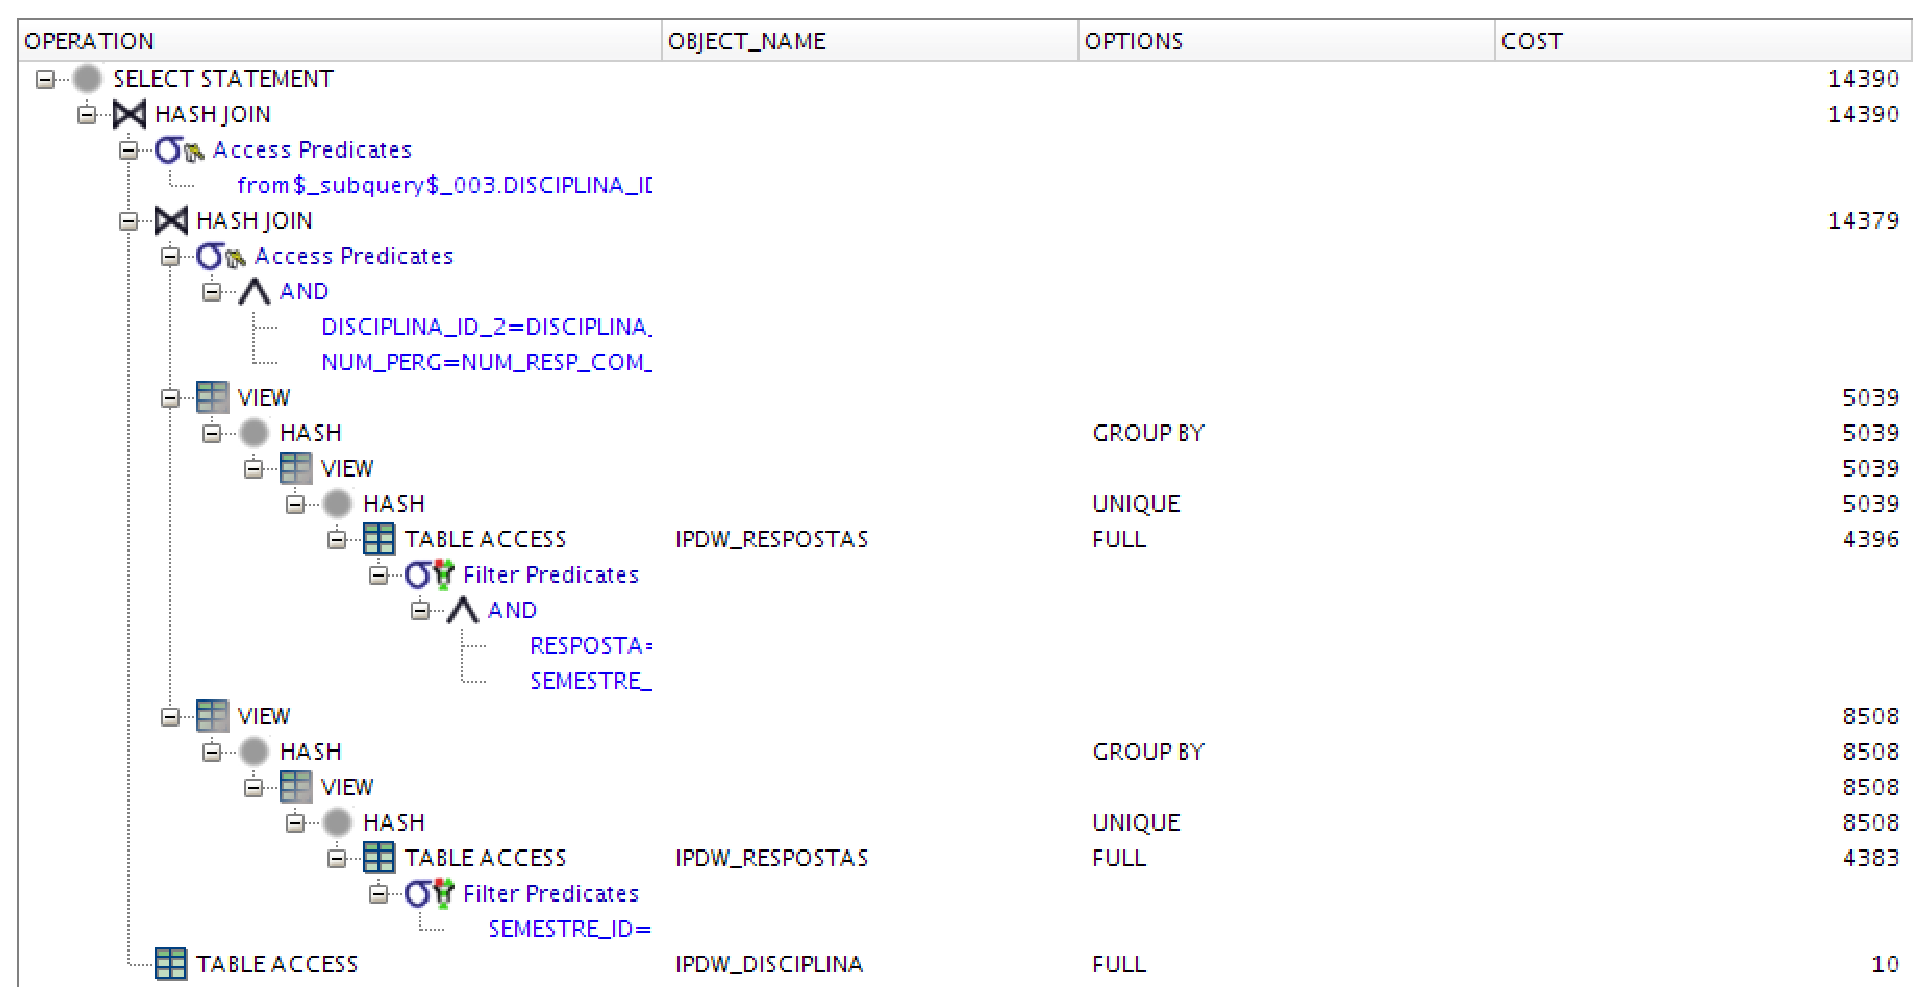
\includegraphics[width=1\textwidth]{4-ii_B}}\\
   \end{center}
   \caption{Plano de execução para a Query \ref{sql:4-ii}.}
   \label{fig:plano_4-ii}
\end{figure}

\begin{figure}[hpt]
   \ContinuedFloat
   \begin{center}
      \subfloat[Situação C]{\label{fig:plano_4-ii_C}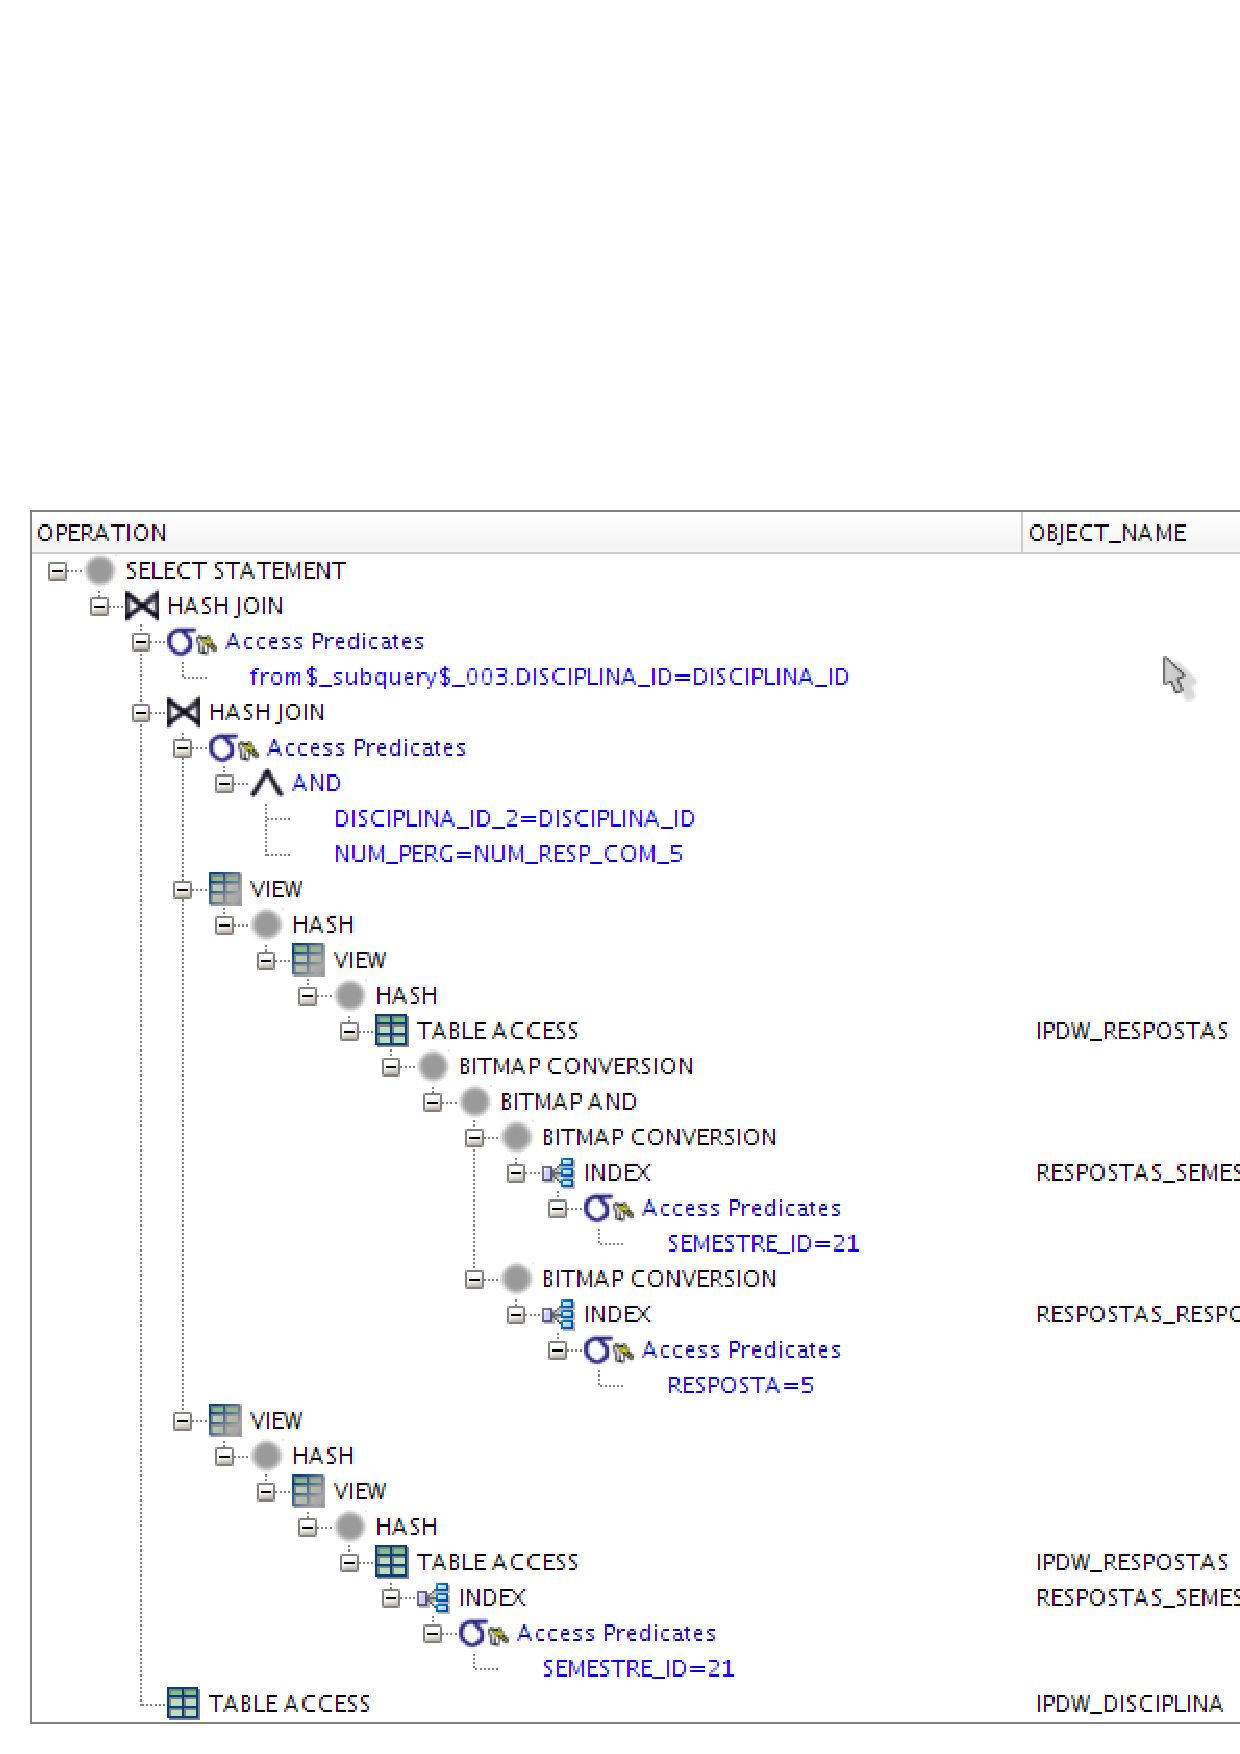
\includegraphics[width=1\textwidth]{4-ii_C}}
   \end{center}
   \caption{Plano de execução para a Query \ref{sql:4-ii}.}
\end{figure}

\begin{table}[hpt]
   \centering
   \begin{tabular}{c c c c}
      \toprule
      \multirow{2}{*}{Query} & \multicolumn{3}{c}{Contexto} \\\cline{2-4}
      & A & B & C \\\midrule
      \ref{sql:1-a} & 0.483 & 0.495 & 0.077 \\\midrule
      \ref{sql:1-b} & 0.639 & 0.517 & 0.019 \\\midrule
      \ref{sql:1-c} & 1.238 & 1.108 & 0.077 \\\midrule
      \ref{sql:2-a} & 1.223 & 1.106 & 0.028 \\\midrule
      \ref{sql:2-b} & 0.781 & 0.654 & 0.638 \\\midrule
      \ref{sql:2-c} & 1.304 & 1.037 & 0.42 \\\midrule
      \ref{sql:3-a-i} & 1.272 & 1.093 & 0.477 \\\midrule
      \ref{sql:3-a-ii} & 313.036 & 235.074 & 242.722 \\\midrule
      \ref{sql:3-b-i} & 2.002 & 1.084 & 0.067 \\\midrule
      \ref{sql:3-b-ii} & 1.885 & 1.064 & 0.046 \\\midrule
      \ref{sql:4-i} & 8.903 & 4.178 & 4.551 \\\midrule
      \ref{sql:4-ii} & 2.039 & 1.199 & 0.753 \\\bottomrule
   \end{tabular}
   \caption{Tempo de execução (segundos) das queries nos contextos A, B e C.}
   \label{tab:tempo}
\end{table}

\end{document}
